\documentclass[12pt]{article}
\usepackage{graphicx}
\usepackage[margin=2cm]{geometry}
\usepackage[utf8]{inputenc}
\usepackage{tikz}
\usepackage[export]{adjustbox}
\usepackage{indentfirst}
\usepackage{wrapfig}
\usepackage{listings}
\usepackage{color}
\usepackage{enumerate}
\usepackage{amssymb, bm}
\usepackage{amsmath}
\usepackage{csvsimple}
\usepackage{tikz}
\usetikzlibrary{positioning}
\usepackage{lscape}
\newcommand\tab[1][1cm]{\hspace*{#1}}
\definecolor{mygreen}{rgb}{0,0.6,0}
\definecolor{mygray}{rgb}{0.5,0.5,0.5}
\definecolor{mymauve}{rgb}{0.58,0,0.82}
\lstset{ %
    backgroundcolor=\color{gray!10!white},
  basicstyle=\tiny, %footnotesize,        % the size of the fonts that are used for the code
  breakatwhitespace=false,         % sets if automatic breaks should only happen at whitespace
  breaklines=true,                 % sets automatic line breaking
  captionpos=b,                    % sets the caption-position to bottom
  commentstyle=\color{mygreen},    % comment style
  deletekeywords={...},            % if you want to delete keywords from the given language
  escapeinside={\%*}{*)},          % if you want to add LaTeX within your code
  extendedchars=true,              % lets you use non-ASCII characters; for 8-bits encodings only, does not work with UTF-8
  frame=single,	                   % adds a frame around the code
  keepspaces=true,                 % keeps spaces in text, useful for keeping indentation of code (possibly needs columns=flexible)
  keywordstyle=\color{blue},       % keyword style
  language=Python,                 % the language of the code
  morekeywords={*,...},           % if you want to add more keywords to the set
  numbers=left,                    % where to put the line-numbers; possible values are (none, left, right)
  numbersep=10pt,                   % how far the line-numbers are from the code
  numberstyle=\tiny\color{mygray}, % the style that is used for the line-numbers
  rulecolor=\color{black},         % if not set, the frame-color may be changed on line-breaks within not-black text (e.g. comments (green here))
  showspaces=false,                % show spaces everywhere adding particular underscores; it overrides 'showstringspaces'
  showstringspaces=false,          % underline spaces within strings only
  showtabs=false,                  % show tabs within strings adding particular underscores
  stepnumber=1,                    % the step between two line-numbers. If it's 1, each line will be numbered
  stringstyle=\color{mymauve},     % string literal style
  tabsize=1,	                   % sets default tabsize to 2 spaces
  title=\lstname                   % show the filename of files included with \lstinputlisting; also try caption instead of title
}
\graphicspath{ }
\usetikzlibrary{arrows}
\usepackage{titlesec}

\titleformat{\section}
  {\normalfont\fontsize{14}{15}\bfseries}{\thesection}{1em}{}
\titleformat{\subsection}
  {\normalfont\fontsize{12}{15}\bfseries}{\thesection}{1em}{}

\title{\textbf{COMP0085 Summative Assignment}}
%\author{Jian Shu (James) Wu \\ }
\date{Jan 6, 2023}

\begin{document}
\maketitle
\section*{Question 1: A biochemical pathway}

\subsection*{(a)} We are given that:

\begin{itemize}
    \item The concentrations of both species B and C depend on that of A.
    \item Molecule C seems to redirect the process that produces enzyme D to produce enzyme E instead.
    \item D catalyses the production of F from B, while E catalyses the production of H from G.
    \item F and H then combine to form the end product I.
\end{itemize}

The corresponding directed acyclic graph:

\begin{center}
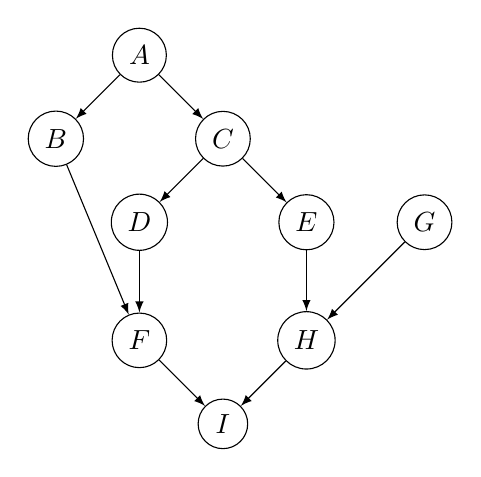
\begin{tikzpicture}[node distance={15mm}, main/.style = {draw, circle}]
    \node[main] (A) {$A$};
    \node[main] (B) [below left of=A] {$B$};
    \node[main] (C) [below right of=A] {$C$};
    \node[main] (E) [below right of=C] {$E$};
    \node[main] (D) [below left of=C] {$D$};
    \node[main] (H) [below of=E] {$H$};
    \node[main] (G) [right of=E] {$G$};
    \node[main] (I) [below left of=H] {$I$};
    \node[main] (F) [above left of=I] {$F$};

    \draw[-latex] (A) -- (B);
    \draw[-latex] (A) -- (C);
    \draw[-latex] (B) -- (F);
    \draw[-latex] (C) -- (D);
    \draw[-latex] (C) -- (E);
    \draw[-latex] (G) -- (H);
    \draw[-latex] (D) -- (F);
    \draw[-latex] (E) -- (H);
    \draw[-latex] (F) -- (I);
    \draw[-latex] (H) -- (I);
\end{tikzpicture}
\end{center}

\newpage


\subsection*{(b)} The moralised graph:

\begin{center}
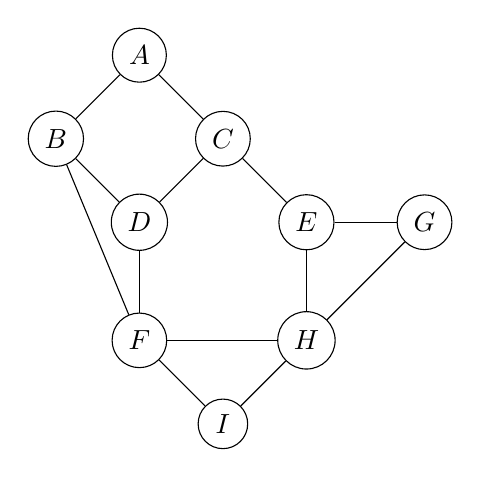
\begin{tikzpicture}[node distance={15mm}, main/.style = {draw, circle}]
    \node[main] (A) {$A$};
    \node[main] (B) [below left of=A] {$B$};
    \node[main] (C) [below right of=A] {$C$};
    \node[main] (E) [below right of=C] {$E$};
    \node[main] (D) [below left of=C] {$D$};
    \node[main] (H) [below of=E] {$H$};
    \node[main] (G) [right of=E] {$G$};
    \node[main] (I) [below left of=H] {$I$};
    \node[main] (F) [above left of=I] {$F$};

    \draw (A) -- (B);
    \draw (A) -- (C);
    \draw (B) -- (F);
    \draw (B) -- (D);
    \draw (C) -- (D);
    \draw (C) -- (E);
    \draw (E) -- (G);
    \draw (G) -- (H);
    \draw (D) -- (F);
    \draw (E) -- (H);
    \draw (F) -- (H);
    \draw (F) -- (I);
    \draw (H) -- (I);
\end{tikzpicture}
\end{center}


An effective triangulation:


\begin{center}
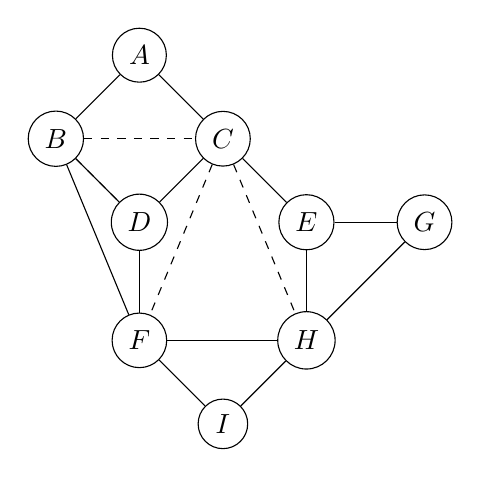
\begin{tikzpicture}[node distance={15mm}, main/.style = {draw, circle}]
    \node[main] (A) {$A$};
    \node[main] (B) [below left of=A] {$B$};
    \node[main] (C) [below right of=A] {$C$};
    \node[main] (E) [below right of=C] {$E$};
    \node[main] (D) [below left of=C] {$D$};
    \node[main] (H) [below of=E] {$H$};
    \node[main] (G) [right of=E] {$G$};
    \node[main] (I) [below left of=H] {$I$};
    \node[main] (F) [above left of=I] {$F$};

    \draw (A) -- (B);
    \draw (A) -- (C);
    \draw (B) -- (F);
    \draw (B) -- (D);
    \draw (C) -- (D);
    \draw (C) -- (E);
    \draw (E) -- (G);
    \draw (G) -- (H);
    \draw (D) -- (F);
    \draw (E) -- (H);
    \draw (F) -- (H);
    \draw (F) -- (I);
    \draw (H) -- (I);

    \draw[dashed] (C) -- (H);
    \draw[dashed] (C) -- (F);
    \draw[dashed] (B) -- (D);
    \draw[dashed] (B) -- (C);

\end{tikzpicture}
\end{center}

where the dashed lines are edges added to triangulate the moralised graph.
\newpage


The resulting junction tree:

\begin{center}
\begin{tikzpicture}[node distance={15mm}, main/.style = {draw, circle}, square/.style={regular polygon,regular polygon sides=4}]
    \node[main] (ABC) {$ABC$};
    \node[square] (BC) [square,draw] [below of=ABC] {$BC$};
    \node[main] (BCDF) [below of=BC] {$BCDF$};
    \node[square] (CF) [square,draw] [below of=BCDF] {$CF$};
    \node[main] (CFH) [below of=CF] {$CFH$};
    \node[square] (FH) [square,draw] [below left of=CFH] {$FH$};
    \node[main] (FHI) [below left of=FH] {$FHI$};
    \node[square] (CH) [square,draw] [below right of=CFH] {$CH$};
    \node[main] (CEH) [below right of=CH] {$CEH$};
    \node[square] (EH) [square,draw] [below of=CEH] {$EH$};
    \node[main] (EGH) [below of=EH] {$EGH$};
    \draw (ABC) -- (BC);
    \draw (BC) -- (BCDF);
    \draw (BCDF) -- (CF);
    \draw (CF) -- (CFH);
    \draw (CFH) -- (FH);
    \draw (FH) -- (FHI);
    \draw (CFH) -- (CH);
    \draw (CH) -- (CEH);
    \draw (CEH) -- (EH);
    \draw (EGH) -- (EH);
\end{tikzpicture}
\end{center}

where the circular nodes are cliques and the square nodes are separators/factors.


The junction tree redrawn as a factor graph:

\begin{center}
\begin{tikzpicture}[node distance={10mm}, main/.style = {draw, circle}, square/.style={fill=black, regular polygon,regular polygon sides=4}]
    \node[main] (A) {$A$};
    \node[square] (ABC) [square,draw] [below of=A];
    \node[main] (B) [below left of=ABC] {$B$};
    \node[main] (C) [below right of=ABC] {$C$};
    \node[square] (BCDF) [square,draw] [below left of=C];
    \node[square] (CEH) [right of=C];
    \node[main] (E) [above right of=CEH] {$E$};
    \node[square] (GEH) [below right of=E];
    \node[main] (G) [right of=GEH] {$G$};
    \node[main] (D) [below left of=BCDF] {$D$};
    \node[square] (CFH) [below right of=C];
    \node[main] (H) [right of=CFH] {$H$};
    \node[square] (FHI) [below left of = H];
    \node[main] (I) [below right of=FHI] {$I$};
    \node[main] (F) [below right of=BCDF] {$F$};

    \draw (ABC) -- (A);
    \draw (ABC) -- (C);
    \draw (ABC) -- (B);
    \draw (BCDF) -- (B);
    \draw (BCDF) -- (C);
    \draw (BCDF) -- (D);
    \draw (BCDF) -- (F);
    \draw (CEH) -- (C);
    \draw (CEH) -- (E);
    \draw (CEH) -- (H);
    \draw (GEH) -- (G);
    \draw (GEH) -- (E);
    \draw (GEH) -- (H);
    \draw (CFH) -- (C);
    \draw (CFH) -- (F);
    \draw (CFH) -- (H);
    \draw (FHI) -- (F);
    \draw (FHI) -- (H);
    \draw (FHI) -- (I);
\end{tikzpicture}
\end{center}
\newpage


\subsection*{(c)}

\begin{center}
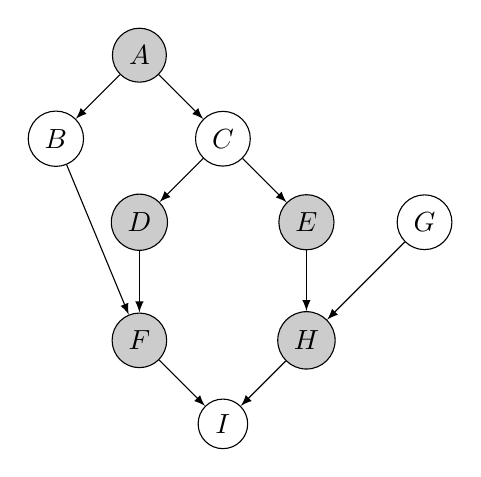
\begin{tikzpicture}[node distance={15mm}, main/.style = {draw, circle}]
    \node[main] (A) [fill=black!20] {$A$};
    \node[main] (B) [below left of=A] {$B$};
    \node[main] (C) [below right of=A] {$C$};
    \node[main] (E) [below right of=C, fill=black!20] {$E$};
    \node[main] (D) [below left of=C, fill=black!20] {$D$};
    \node[main] (H) [below of=E, fill=black!20] {$H$};
    \node[main] (G) [right of=E] {$G$};
    \node[main] (I) [below left of=H] {$I$};
    \node[main] (F) [above left of=I, fill=black!20] {$F$};

    \draw[-latex] (A) -- (B);
    \draw[-latex] (A) -- (C);
    \draw[-latex] (B) -- (F);
    \draw[-latex] (C) -- (D);
    \draw[-latex] (C) -- (E);
    \draw[-latex] (G) -- (H);
    \draw[-latex] (D) -- (F);
    \draw[-latex] (E) -- (H);
    \draw[-latex] (F) -- (I);
    \draw[-latex] (H) -- (I);
\end{tikzpicture}
\end{center}


The set $\{A, D, E, F, H\}$ is a non-unique smallest set of molecules such that if the concentrations of the species within the set are known, the concentrations of the others $\{B, C, G, I\}$ would all be independent (conditioned on the measured ones).


\subsection*{(d)}

Using our factor analysis model, we can describe the biochemical pathway as:

\[\delta[\textbf{x}] = \Lambda \textbf{z} + \epsilon\]

where $\delta[\textbf{x}]$ are the concentration perturbations, $\epsilon \sim \mathcal{N} (0, \Psi)$ are the reaction specific Gaussian noise variables, \Lambda is the factor loading matrix, and $z \sim \mathcal{N} (0, I)$ are the latent factors, the parent concentration perturbations.

From the graph structure, we know that:

\[\Lambda = \begin{bmatrix}
                 0 & 0 & 0 & 0 & 0 & 0 & 0 & 0 & 0  \\
                 \Lambda_{BA} & 0 & 0 & 0 & 0 & 0 & 0 & 0 & 0  \\
                 \Lambda_{CA} & 0 & 0 & 0 & 0 & 0 & 0 & 0 & 0  \\
                 0 & 0 & \Lambda_{DC} & 0 & 0 & 0 & 0 & 0 & 0  \\
                 0 & 0 & \Lambda_{EC} & 0 & 0 & 0 & 0 & 0 & 0  \\
                 0 & \Lambda_{FB} & 0 & \Lambda_{FD} & 0 & 0 & 0 & 0 & 0  \\
                 0 & 0 & 0 & 0 & 0 & 0 & 0 & 0 & 0  \\
                 0 & 0 & 0 & 0 & \Lambda_{HE} & 0 & \Lambda_{HG} & 0 & 0  \\
                 0 & 0 & 0 & 0 & 0 & \Lambda_{IF} & 0 & \Lambda_{IH} & 0 \\
         \end{bmatrix} \text{ and }
    \textbf{z} = \begin{bmatrix}
                 z_A  \\
                 z_B  \\
                 z_C  \\
                 z_D  \\
                 z_E  \\
                 z_F  \\
                 z_G  \\
                 z_H  \\
                 z_I \\
         \end{bmatrix}
\]

Having observations for $\delta[B]$, $\delta[D]$, $\delta[E]$ and $\delta[G]$:

\[
\begin{bmatrix}
                 \delta[B]  \\
                 \delta[D]  \\
                 \delta[E]  \\
                 \delta[G]  \\
         \end{bmatrix} = \begin{bmatrix}
                 \Lambda_{BA} & 0 & 0 & 0 & 0 & 0 & 0 & 0 & 0  \\
                 0 & 0 & \Lambda_{DC} & 0 & 0 & 0 & 0 & 0 & 0  \\
                 0 & 0 & \Lambda_{EC} & 0 & 0 & 0 & 0 & 0 & 0  \\
                 0 & 0 & 0 & 0 & 0 & 0 & 0 & 0 & 0  \\
         \end{bmatrix} \begin{bmatrix}
                 z_A  \\
                 z_B  \\
                 z_C  \\
                 z_D  \\
                 z_E  \\
                 z_F  \\
                 z_G  \\
                 z_H  \\
                 z_I \\
         \end{bmatrix} +  \begin{bmatrix}
                 \epsilon_B  \\
                 \epsilon_D  \\
                 \epsilon_E  \\
                 \epsilon_G  \\
         \end{bmatrix}
\]

Knowing \textbf{z} are the parent concentration perturbations, we can see that these simplify to a factor analysis set up:

\[
    \begin{bmatrix}
                 \delta[B]  \\
                 \delta[D]  \\
                 \delta[E]  \\
         \end{bmatrix} = \begin{bmatrix}
                 \Lambda_{BA} & 0   \\
                 0 & \Lambda_{DC} \\
                 0 & \Lambda_{EC} \\
         \end{bmatrix} \begin{bmatrix}
                 \delta[A]  \\
                 \delta[C]  \\
         \end{bmatrix} +  \begin{bmatrix}
                 \epsilon_B  \\
                 \epsilon_D  \\
                 \epsilon_E  \\
         \end{bmatrix}
\]

Thus, we would expect to recover the factors of $A$ and $C$, $\delta[A]$ and $\delta[C]$, the two parent nodes of the observations.


\subsection*{(e)}

From factor analysis, we would recover $\delta[A]$ and $\delta[C]$.
In theory, if these concentration perturbations had unknown parent factors, we could use the results to recover the concentration perturbations of those parent features.
However, in our DAG this is not the case, so we would not be able to recover any other species in the cascade because  they are all downstream from the known concentration perturbations and those recovered from factor analysis.
Similarly, the downstream weights in the DAG from the known measurements would also be unidentifiable.
Using factor analysis, we would only be able to identify the upstream weights from the measurements, up to an unknown scale factor.
These are the weights $\Lambda_{BA}$, $\Lambda_{DC}$, and $\Lambda_{EC}$.
Moreover, knowing $\delta[C]$ from factor analysis, we would also be able to determine $\Lambda_{CA}$, up to an unknown scale factor.


\newpage
\section*{Question 2: Bayesian linear and Gaussian process regression}

\subsection*{(a)}

We want the posterior mean and covariance over $a$ and $b$.
Defining a weight vector $\textbf{w}$:
\[\textbf{w} = \begin{bmatrix}
                 a \\
                 b
         \end{bmatrix}\]

Our distribution for $\textbf{w}$:
\[P(\textbf{w}) = \mathcal{N}(\mu_{\textbf{w}}, \Sigma_{\textbf{w}}) = \mathcal{N} \left(
\begin{bmatrix}
                 \mu_a \\
                 \mu_b
         \end{bmatrix} ,
\begin{bmatrix}
                 \sigma_a^2 & 0 \\
                 0 & \sigma_b^2
         \end{bmatrix}
\right)

\]


For our data $\mathcal{D} = \{\textbf{X}, \textbf{y}\}$:
\[P(\mathcal{D} | \textbf{w}) = \prod_{t=1}^{T}\mathcal{N} \left( y_t - \textbf{w}^T \textbf{x}_t, \sigma^2
\right)
\]

where $\textbf{x}_t =  \begin{bmatrix}
                 t_1 \\
                 1
         \end{bmatrix} \in  \mathbb{R}^{2 \times 1}$ and $y_t \in \mathbb{R}^{1 \times 1}$ our response $f_{obs}(t_1)$.

Knowing:
\[P(\textbf{w} | \mathcal{D}) \propto P(\mathcal{D} | \textbf{w}) P(\textbf{w})\]

we can substitute the above distributions:
\[P(\textbf{w} | \mathcal{D}) \propto
  \exp \left(\frac{-1}{2 \sigma^2} \left( \textbf{y} - \textbf{w}^T \textbf{X}\right) \left( \textbf{y} - \textbf{w}^T \textbf{X}\right)^T \right)
\exp \left(\frac{-1}{2} \left( \textbf{w} -\mu_{\textbf{w}}\right)^T \Sigma_{\textbf{w}}^{-1} \left( \textbf{w} -\mu_{\textbf{w}}\right)\right)
\]

where $\textbf{X} =  \begin{bmatrix}
                 t_1 & t_2 \cdots t_T \\
                 1 & 1 \cdots 1
         \end{bmatrix} \in  \mathbb{R}^{2 \times T}$ and $\textbf{y} \in \mathbb{R}^{1 \times T}$.
Expanding:

\[\log P(\textbf{w} | \mathcal{D}) \propto
  \frac{-1}{2} \left( \frac{\textbf{y} \textbf{y}^T}{\sigma^2} - 2\textbf{w}^T \frac{\textbf{X}\textbf{y}^T}{\sigma^2} + \textbf{w}^T \frac{\textbf{X} \textbf{X}^T}{\sigma^2} \textbf{w} +  \textbf{w}^T \Sigma_{\textbf{w}}^{-1}  \textbf{w} - 2\textbf{w}^T \Sigma_{\textbf{w}}^{-1}\mu_{\textbf{w}} + \mu_{\textbf{w}}^T\Sigma_{\textbf{w}}^{-1}\mu_{\textbf{w}} \right)
\]

collecting $\textbf{w}$:
\[\log P(\textbf{w} | \mathcal{D}) \propto
  \frac{-1}{2} \left( \textbf{w}^T \left(\frac{\textbf{X} \textbf{X}^T}{\sigma^2} + \Sigma_{\textbf{w}}^{-1} \right)  \textbf{w} - 2\textbf{w}^T \left(\frac{\textbf{X}\textbf{y}^T}{\sigma^2} + \Sigma_{\textbf{w}}^{-1} \mu_{\textbf{w}}\right)  \right)
\]

Knowing that the posterior $P(\textbf{w} | \mathcal{D})$ will be Gaussian with mean $\bar{\mu}_{\textbf{w}}$ and covariance $\bar{\Sigma}_{\textbf{w}}$, we can see that expanding the exponent component of a Gaussian would have the form:

\[\left( \textbf{w} - \bar{\mu}_{\textbf{w}} \right)^T \bar{\Sigma}_{\textbf{w}}^{-1} \left( \textbf{w} - \bar{\mu}_{\textbf{w}} \right) = \textbf{w}^T \bar{\Sigma}_{\textbf{w}}^{-1} \textbf{w} -2 \textbf{w}^T \bar{\Sigma}_{\textbf{w}}^{-1} \bar{\mu}_{\textbf{w}} + \bar{\mu}_{\textbf{w}}^T \bar{\Sigma}_{\textbf{w}}^{-1} \bar{\mu}_{\textbf{w}}\]

Thus we can identify the posterior covariance:
\[\bar{\Sigma}_{\textbf{w}} = \left(\frac{\textbf{X} \textbf{X}^T}{\sigma^2} + \Sigma_{\textbf{w}}^{-1} \right)^{-1}\]

and the posterior mean:
\[\bar{\mu}_{\textbf{w}} = \bar{\Sigma}_{\textbf{w}} \left(\frac{\textbf{X}\textbf{y}^T}{\sigma^2} + \Sigma_{\textbf{w}}^{-1} \mu_{\textbf{w}}\right) \]


\newpage
Computing the posterior mean and covariance over $a$ and $b$ given by the $CO_2$ data:


\begin{figure}[h]
\centering
\begin{minipage}{.5\textwidth}
  \centering
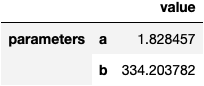
\includegraphics[scale = 0.5]{outputs/q2/a-mean}
\caption{The Posterior Mean}
\label{fig:fig2-a-mean}
\end{minipage}%
\begin{minipage}{.5\textwidth}
  \centering
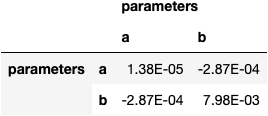
\includegraphics[scale = 0.5]{outputs/q2/a-covariance}
\caption{The Posterior Covariance}
\label{fig:fig2-a-covariance}
\end{minipage}
\end{figure}

\subsection*{(b)}

Plotting the residuals $g_{obs}(t) = f_{obs}(t) - (a_{MAP}t + b_{MAP})$:

\begin{figure}[h]
\centering
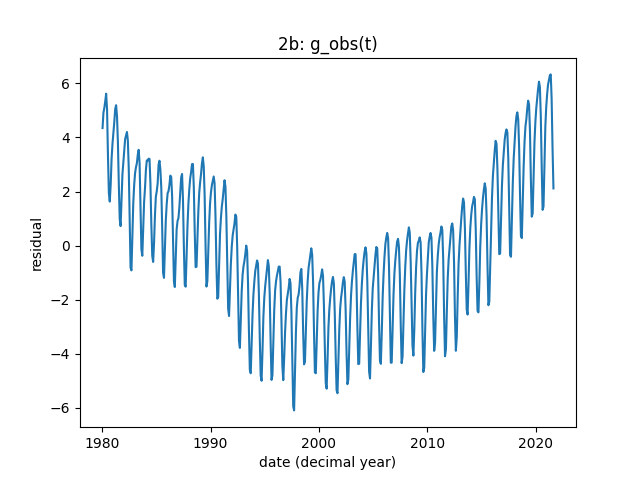
\includegraphics[scale=0.5]{outputs/q2/b-residuals-timeseries}
\caption{$g_{obs}(t)$}
\label{fig:b-residuals-timeseries}
\end{figure}

\begin{figure}[h]
\centering
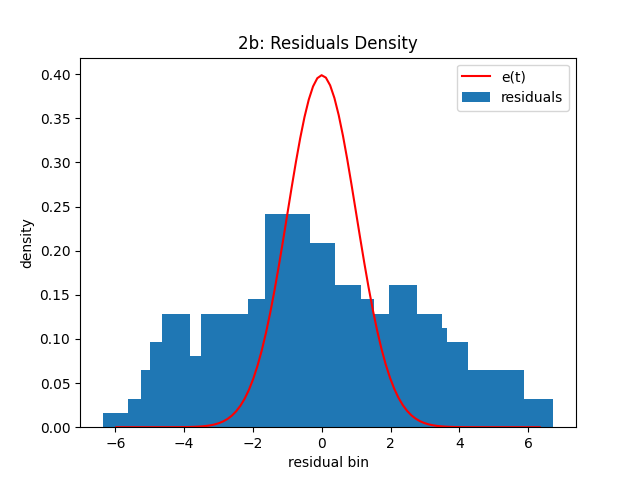
\includegraphics[scale=0.5]{outputs/q2/b-residuals-density-estimation}
\caption{Density Estimation of Residuals vs $e(t) \sim \mathcal{N}(0, 1)$}
\label{fig:b-residuals-density-estimation}
\end{figure}

We can see that the residuals do not perfectly conform to our prior over $e(t) \sim \mathcal{N}(0, 1)$.
The density estimation shows that a mean of zero is a reasonable prior belief however the data does not seem to exhibit unit variance.
Also, observing $g_{obs}(t)$ we see that there is periodic structure in the timeseries meaning that the data is not independently and identically distributed as $e(t) \sim \mathcal{N}(0, 1)$ would suggest.
If this were the case, we would expect $g(t)$ to look like random noise.

\newpage
\subsection*{(c \& d)}

We are considering the kernel:

\[k(s, t) = \theta^2 \exp\left( - \frac{2\sin^2(\pi(s-t)/\tau)}{\sigma^2}\right) + \phi^2 \exp\left( - \frac{(s-t)^2}{2\eta^2}\right) + \zeta^2 \delta_{s=t}\]

We can make qualitative observations of this kernel by visualising the covariance (gram) matrix:

\begin{figure}[h]
\centering
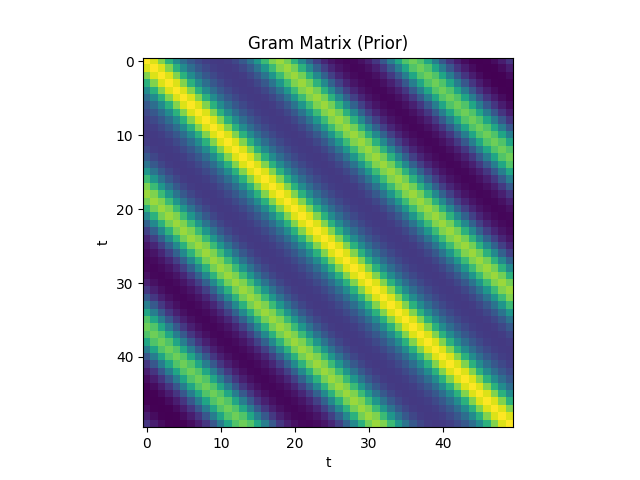
\includegraphics[scale=0.5]{outputs/q2/c-gram-matrix}
\caption{Covariance Matrix}
\label{fig:c-gram-matrix}
\end{figure}

We can observe a striped pattern which indicate higher covariance at regular intervals.
This can be attributed to the sinusoidal term in the kernel and encourages periodic structure in functions.
Additionally, we can see that covariance values also decay as they are further away from the diagonal.
This can be attributed to the exponential term in the kernel, encouraging points closer in time to be more correlated and vice versa.
From visualising $g(t)$, we would want to model this with a class of functions which exhibit both of these behaviours as $g(t)$ looks periodic (seasonal with respect to each year) and locally correlated (smooth).

We can also visualise some samples from a Gaussian Process with the same covariance matrix and zero mean.
This verifies our observations about the covariance matrix.

\begin{figure}[h]
\centering
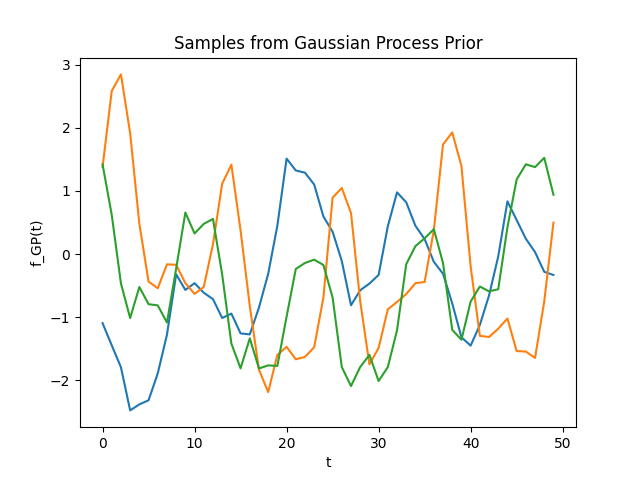
\includegraphics[scale=0.5]{outputs/q2/c-samples}
\caption{Samples from a zero mean GP with the provided covariance kernel}
\label{fig:c-samples}
\end{figure}

\newpage
More specifically, we can see how changing each hyper-parameter will affect the characteristics of the function.

\begin{figure}[h]
\centering
\begin{minipage}{.5\textwidth}
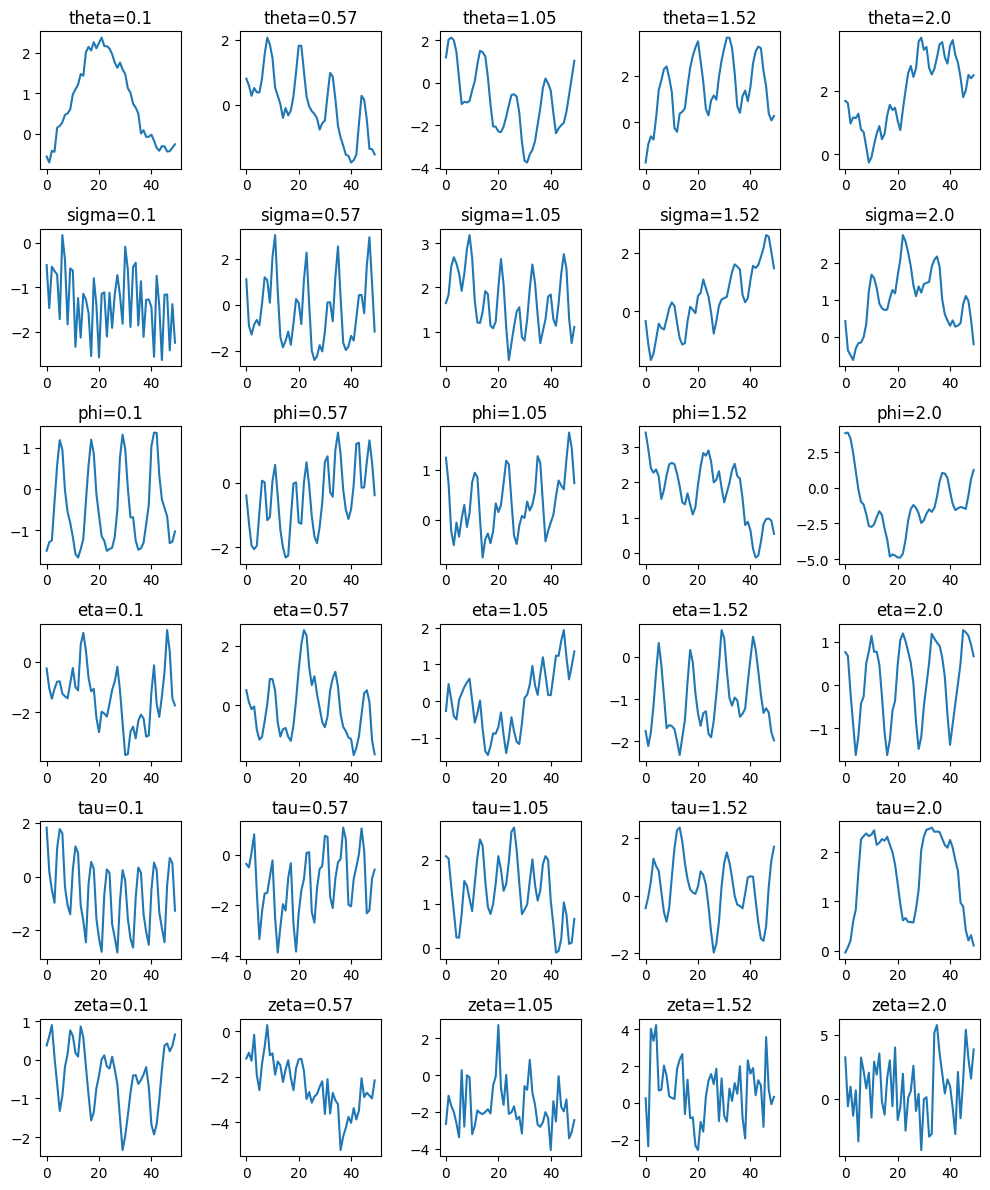
\includegraphics[scale = 0.35]{outputs/q2/c-parameter-samples}
\caption{Samples for different parameters}
\label{fig:fig2-c-parameter-samples}
  \centering
\end{minipage}%
\begin{minipage}{.5\textwidth}
  \centering
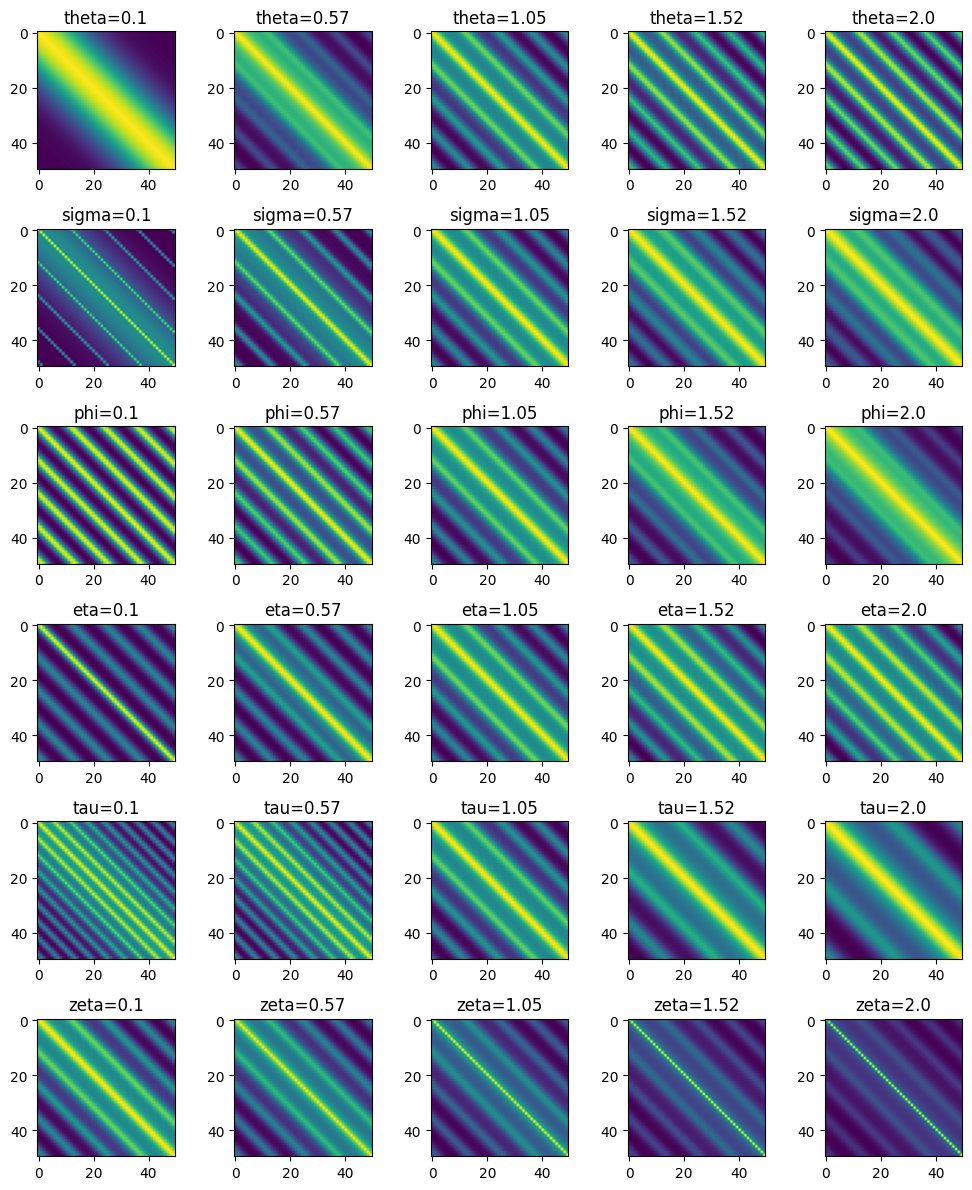
\includegraphics[scale = 0.35]{outputs/q2/c-parameter-grams}
\caption{Covariances for different parameters}
\label{fig:fig2-c-parameter-grams}
\end{minipage}
\end{figure}

\begin{itemize}
\item [$\theta$:] As $\theta$ increases, we see more pronounced periodic behavior in the sample function by increasing its amplitude.
    The covariance matrix shows how increasing $\theta$ visually reveals the striped periodic component.
        This is expected because it is the parameter that adjusts the amplitude of the periodic component.
\item [$\sigma$:] As $\sigma$ increases, we see smoother periodic behaviour in the sample function.
    The covariance matrix shows how increasing $\sigma$ will increase covariance values around each periodic stripe of the covariance matrix.
    This is expected because it adjusts the lengthscale of the periodic portion of the kernel.
\item [$\phi$:] As $\phi$ increases, we see the ratio of the amplitude of the periodicity component of the sample function reduces compared to the baseline.
    The covariance matrix shows how increasing $\phi$ will start to increase the non-periodic component masking the periodic stripes.
    This is expected because it adjusts the weight of the squared exponential portion of the kernel.
    The periodic component remains the same (i.e.same amplitude) but the large baseline shifts from increasing $\phi$ ends up dominating the function visually.
\item [$\eta$:] As $\eta$ increases we see smoother sample functions.
This is expected because the $\eta$ increases the lengthscale of the squared exponential component, allowing for smoother functions.
This causes the off-diagonals of the gram matrix to increase, however the periodic component is still maintained because $\eta$ doesn't affect the relative weighting between the two components.
\item [$\tau$:] As $\tau$ increases, the period of the periodic function increases.
We can see this reflected in the stripes in the gram matrix getting further apart and the period of the samples.
This makes sense because we are adjusting the period parameter in the sinusoid function of the periodic term.
\item [$\zeta$:] As $\zeta$ increases, the function becomes less smooth.
    This is because the $\zeta$ parameter adjusts the weight of the $\delta_{s=t}$ kernel.
    This places stronger emphasis on the independence of each timestep, which can be seen with the reduction of relative magnitude of off-diagonals in the gram matrix.
    This masks the periodic and squared-exponential components as we can see with the increased magnitude of the functions as $\zeta$ increases.
\end{itemize}
\subsection*{(e)}
Suitable values for hyper-parameters can be chosen through a combination of visual inspection and prior knowledge.
For example, it is a reasonable assumption that the $CO_2$ concentration levels have a strong yearly seasonality behaviour due to the cyclic changes in temperature, humidity, etc.
This behaviour cannot be modelled by our Bayesian linear regression and is reflected in our residuals $g(t)$.
Thus we can choose $\tau=1$ to ensure functions with a period of one year to reflect this prior knowledge.
It can be difficult to quantitatively choose values for the other parameters as they can relate to the uncertainty exhibited in the data (i.e. the smoothness of the function).
One approach is to maximise:

\[\log P(\textbf{y} | \textbf{X}) = -\frac{1}{2} \textbf{y}^T (\textbf{K} + \sigma^2\textbf{I})^{-1} \textbf{y} - \frac{1}{2} \log |\textbf{K}+ \sigma^2\textbf{I}| - \frac{n}{2}\log(2\pi)\]

the log-likelihood  of the posterior distribution with respect to the given data where $\textbf{K}$ is the gram matrix for the kernel (equation 2.30 from http://gaussianprocess.org/gpml/chapters/RW2.pdf).
We define a loss function as the negative log-likelihood and employ gradient-based algorithms to find optimal values for these parameters.

Comparing the hyperparameters corresponding to before and after training side by side:

\begin{figure}[h]
\centering
\begin{minipage}{.5\textwidth}
  \centering
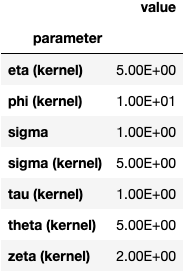
\includegraphics[scale=0.5]{outputs/q2/f-untrained-parameters}
\caption{Untrained hyperparameters}
\label{fig:f-untrained-parameters}
\end{minipage}%
\begin{minipage}{.5\textwidth}
  \centering
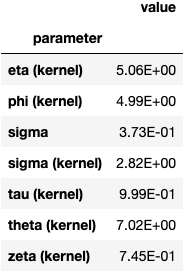
\includegraphics[scale=0.5]{outputs/q2/f-trained-parameters}
\caption{Trained Hyperparmaeters}
\label{fig:f-trained-parameters}
\end{minipage}
\end{figure}

We can analyse some of the changes in these parameters from optimisation to gain some insights.
We can see that $\tau$ remains the same as we would expect, given the yearly seasonality we knew apriori.
On the other hand, the value for $\zeta$ is significantly reduced signifying that $\delta_{s=t}$ is not a very good kernel for representing the data as datapoints at different timesteps do exhibit correlations and are not independently and identically distributed.

\newpage
\subsection*{(f)}
Extrapolating the $CO_2$ concentration levels using both the untrained and trained hyperparameters:

\begin{figure}[h]
\centering
\begin{minipage}{.5\textwidth}
  \centering
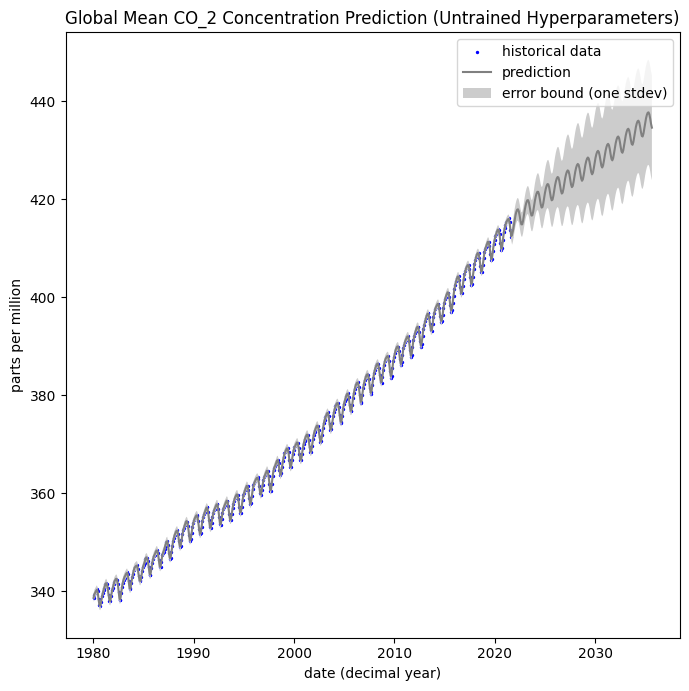
\includegraphics[scale=0.5]{outputs/q2/f-extrapolation-untrained}
\caption{Untrained extrapolation}
\label{fig:f-extrapolation-untrained}
\end{minipage}%
\begin{minipage}{.5\textwidth}
  \centering
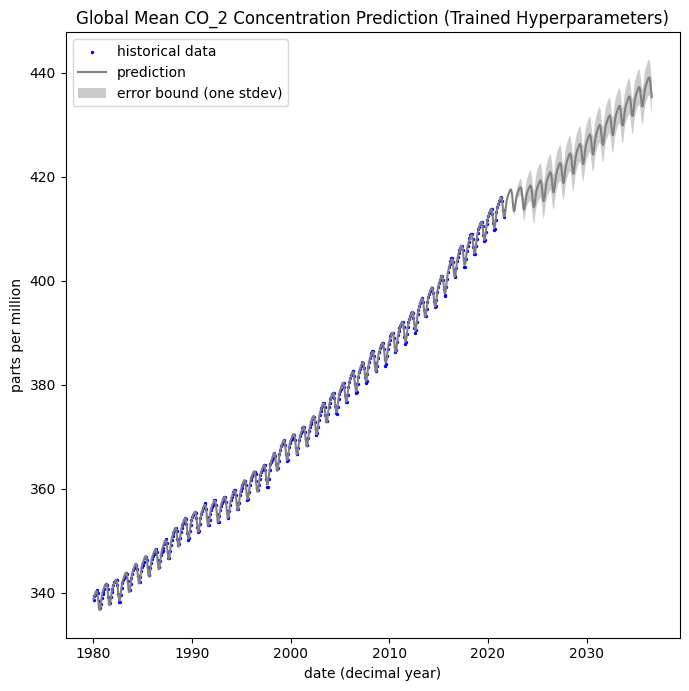
\includegraphics[scale=0.5]{outputs/q2/f-extrapolation-trained}
\caption{Trained extrapolation}
\label{fig:f-extrapolation-trained}
\end{minipage}
\end{figure}

We can see that the extrapolation shows a continued increase in $CO_2$ in the future.
This follows our expectations given that the levels has been steadily increasing in the past and our Bayesian linear regression model assumption.
Moreover, the concentration continues to exhibit yearly seasonality (for the trained extrapolation) as we would expect through the choice of our kernel for modelling the residuals $g(t)$.
We can see that the conclusions can be quite sensitive to kernel hyperparameters when comparing the extrapolations from before and after training.
Prior to training, the extrapolated prediction is not representative of the given data, with very large uncertainties.
After training, we can see that the prediction is much more reasonable, and qualitatively the uncertainty bounds seem to exhibit the historical variability in the data.


\subsection*{(g)}

This procedure is not fully Bayesian because despite using a posterior estimate of our linear regression terms, we only use a MAP point estimate when making prediction.
For a fully Bayesian approach, we should also incorporate the uncertainty of the linear regression parameters into our extrapolation/uncertainty bounds.
For our procedure, we only include the uncertainty of $g(t)$ however it can be observed in the plots that the trend is not perfectly linear so this should be reflected in the uncertainty of our extrapolation.
Another approach could be to add a linear kernel to our combined kernel function and model $f(t)$ directly with our kernel, removing the linear regression component in our procedure.
Thus our kernel extrapolation would incorporate the uncertainty of all components of our signal.

\newpage
The Python code for Bayesian Linear Regression:
\lstinputlisting[language=Python]{src/models/bayesian_linear_regression.py}

\newpage
The Python code for kernels:
\lstinputlisting[language=Python]{src/models/kernels.py}

\newpage
The Python code for Gaussian Process Regression:
\lstinputlisting[language=Python]{src/models/gaussian_process_regression.py}

\newpage
The rest of the Python code for question 2:
\lstinputlisting[language=Python]{src/solutions/q2.py}

\newpage
\section*{Question 3: Mean-field learning}

\subsection*{(a)}

The free energy is can be expressed as:
\[\mathcal{F}(q, \theta) = \left\langle \log P(\textbf{x}, \textbf{s} | \theta)\right\rangle_{q(\textbf{s})} + H[Q(\textbf{s})]\]


Knowing,
\[\log P(\textbf{x}, \textbf{s} | \theta) = \log P(\textbf{x} | \textbf{s}, \theta) + \log P(\textbf{s} | \theta)\]

we can write:

\[\mathcal{F}(Q, \theta) = \left\langle \log P(\textbf{x} | \textbf{s}, \theta)\right\rangle_{q(\textbf{s})} + \left\langle \log P(\textbf{s} | \theta)\right\rangle_{q(\textbf{s})} + H\left[ q(\textbf{s})\right] \]

Moreover, our mean field approximation is:
\[q(\textbf{s}) = \prod_{k=1}^{K} q_{k} (s_k) \]


where $q_{k} (s_k) = (\lambda_k)^{s_k} (1-\lambda_k)^{(1-s_k)}$.


Given that:

\[ P(\textbf{x} | \textbf{s}, \theta)  = \mathcal{N}\left( \sum_{k=1}^{K} s_k \mu_k, \sigma^2 \textbf{I} \right)}\]

we can substitute the appropriate terms:

\[ P(\textbf{x} | \textbf{s}, \theta)  = 2\pi^{-\frac{D}{2}} |\sigma^2 \textbf{I}|^{-\frac{1}{2}} \exp \left( -\frac{1}{2} \left(\textbf{x} - \sum_{k=1}^{K} s_k \mu_k\right)^T \frac{1}{\sigma^2} \textbf{I}  \left(\textbf{x} - \sum_{k=1}^{K} s_k \mu_k\right) \right) \]

with $d$ being the number of dimensions.


Taking the logarithm:

\[ \log P(\textbf{x} | \textbf{s}, \theta)  = -\frac{D}{2} \log (2 \pi \sigma^2)  -\frac{1}{2 \sigma^2} \left(\textbf{x}^T\textbf{x} - 2 \textbf{x}^T\sum_{k=1}^{K} s_k \mu_k   + \sum_{k=1}^{K} \sum_{k=1}^{K} s_k s_{k'} \mu_k^T\mu_{k'} \right) \]

The expectation distributed to the relevant terms:

\[
\left\langle \log P(\textbf{x} | \textbf{s}, \theta)\right\rangle_{q(\textbf{s})} \\
= -\frac{D}{2} \log (2 \pi \sigma^2)   -\frac{1}{2 \sigma^2} \left(\textbf{x}^T\textbf{x} - 2 \textbf{x}^T\sum_{k=1}^{K} \left\langle s_k \right\rangle_{q_{k} (s_k)} \mu_k   + \sum_{k=1}^{K} \sum_{k'=1}^{K} \left\langle s_k s_{k'} \right\rangle_{q_{k} (s_k) q_{k'} (s_k')} \mu_k^T\mu_{k'} \right)\]

Evaluating the expectations:

\[
\left\langle \log P(\textbf{x} | \textbf{s}, \theta)\right\rangle_{q(\textbf{s})} \\
= -\frac{D}{2} \log (2 \pi \sigma^2)  -\frac{1}{2 \sigma^2} \left(\textbf{x}^T\textbf{x} - 2 \textbf{x}^T\sum_{k=1}^{K}  \lambda_k  \mu_k   + \sum_{k=1}^{K} \sum_{k'=1, k'\neq k}^{K}  \lambda_k \lambda_{k'} \mu_k^T\mu_{k'} + \sum_{k=1}^{K}  \lambda_k \mu_k^T\mu_k \right)\]

where $\left\langle s_k s_k \right\rangle_{q_{k} (s_k)} = \left\langle s_k \right\rangle_{q_{k} (s_k)}$ because $s_k \in \{0, 1\}$.

Given that:

\[ P(\textbf{s} | \theta) = \prod_{k=1}^{K}\pi_k^{s_k} (1-\pi_k)^{(1-s_k)}\]

Taking the logarithm:

\[ \log P(\textbf{s} | \theta) = \sum_{k=1}^{K}s_k \log \pi_k + (1-s_k) \log (1-\pi_k)}\]

The expectation distributed to the relevant terms:

\[ \left\langle \log P(\textbf{s} | \theta)\right\rangle_{q(\textbf{s})}= \sum_{k=1}^{K} \left\langle s_k \right\rangle_{q_{k} (s_k)} \log \pi_k + (1-\left\langle s_k\right\rangle_{q_{k} (s_k)}) \log (1-\pi_k)}\]

Evaluating the expectations with respect to $q(\textbf{s})$:

\[ \left\langle \log P(\textbf{s} | \theta)\right\rangle_{q(\textbf{s})}= \sum_{k=1}^{K} \lambda_k \log \pi_k + (1-\lambda_k) \log (1-\pi_k)}\]

To compute the third term, we use the mean field factorisation:

\[H\left[ q(\textbf{s})\right] = \sum_{k=1}^K H\left[ q_{k} (s_k)\right] \]

Thus,

\[H\left[ q(\textbf{s})\right] = - \sum_{k=1}^K \sum_{s_k \in \{0, 1\}} q_{k} (s_k) \log q_{k} (s_k) \]

Substituting the appropriate values:

\[H\left[ q(\textbf{s})\right] = - \sum_{k=1}^K \lambda_k \log \lambda_k + (1-\lambda_k) \log (1-\lambda_k) \]

Combining, we have our free energy expression:


\[
\begin{array}{l}
\tab \mathcal{F}(q, \theta) = \\
\tab \tab \frac{-D}{2} \log (2 \pi \sigma^2)   -\frac{1}{2 \sigma^2} \left(\textbf{x}^T\textbf{x} - 2 \textbf{x}^T\sum_{k=1}^{K}  \lambda_k  \mu_k   + \sum_{k=1}^{K} \sum_{k'=1, k'\neq k}^{K}  \lambda_k \lambda_{k'} \mu_k^T\mu_{k'} + \sum_{k=1}^{K}  \lambda_k \mu_k^T\mu_k \right) \\
\tab \tab + \sum_{k=1}^{K} \lambda_k \log \pi_k + (1-\lambda_k) \log (1-\pi_k)}\\
\tab \tab - \sum_{k=1}^K \lambda_k \log \lambda_k + (1-\lambda_k) \log (1-\lambda_k)
\end{array}
\]

To derive the partial update for $q_k(s_k)$ we take the variational derivative of the Lagrangian, enforcing the normalisation of $q_k$:

\[\frac{\partial}{\partial q_k}\left( \mathcal{F}(q, \theta) + \lambda^{LG} \int q_k -1)\right) = \left\langle \log P(\textbf{x}, \textbf{s} | \theta)\right\rangle_{\prod_{k'\neq k} q_{k'}(s_{k'})} - \log q_k(s_k) - 1 + \lambda^{LG}\]

where $\lambda^{LG}$ is the Lagrange multiplier.

Setting this to zero we can solve for the $\lambda_k$ that maximises the free energy:

\[\log q_k(s_k) = \left\langle \log P(\textbf{x}, \textbf{s} | \theta)\right\rangle_{\prod_{k'\neq k} q_{k'}(s_{k'})} - 1 + \lambda^{LG}\]


Similar to our free energy derivation:

\[\left\langle \log P(\textbf{x} |  \textbf{s}, \theta)\right\rangle_{\prod_{k'\neq k} q_{k'}(s_{k'})} \propto  -\frac{1}{2 \sigma^2} \left(\textbf{x}^T\textbf{x} - 2 \textbf{x}^T\sum_{k=1}^{K} \left\langle s_k \right\rangle_{\prod_{k'\neq k} q_{k'}(s_{k'})} \mu_k   + \sum_{k=1}^{K} \sum_{k'=1}^{K} \left\langle s_k s_{k'} \right\rangle_{\prod_{k'\neq k} q_{k'}(s_{k'})} \right)\]

and

\[ \left\langle \log P(\textbf{s} | \theta)\right\rangle_{\prod_{k'\neq k} q_{k'}(s_{k'})} = \sum_{k=1}^{K} \left\langle s_k \right\rangle_{\prod_{k'\neq k} q_{k'}(s_{k'})} \log \pi_k + (1-\left\langle s_k\right\rangle_{\prod_{k'\neq k} q_{k'}(s_{k'})}) \log (1-\pi_k)}\]

We can write:

\[\log q_k(s_k) \propto  \log P(\textbf{x} |  \textbf{s}, \theta)\right\rangle_{\prod_{k'\neq k} q_{k'}(s_{k'})} + \left\langle \log P(\textbf{s} | \theta)\right\rangle_{\prod_{k'\neq k} q_{k'}(s_{k'})} \]

Substituting the relevant terms:

\[\log q_k(s_k) \propto  -\frac{1}{2 \sigma^2} \left( - 2 s_k \textbf{x}^T \mu_k   + s_k s_k  \mu_k^T\mu_k +  2 \sum_{k'=1, k'\neq k}^{K}  s_k \lambda_{k'}  \mu_k^T\mu_{k'}  \right) + s_k \log \pi_k + (1- s_k ) \log (1-\pi_k)}
\]

Knowing $\log q_k(s_k) = s_k \log \lambda_k + (1-s_k) \log (1-\lambda_k)$:

\[\log q_k(s_k) \propto s_k \log \frac{\lambda_k}{1-\lambda_k}\]

Thus,

\[s_k \log \frac{\lambda_k}{1-\lambda_k} \propto  -\frac{1}{2 \sigma^2} \left( - 2 s_k \textbf{x}^T \mu_k   + s_k s_k  \mu_k^T\mu_k +  2 \sum_{k'=1, k'\neq k}^{K}  s_k \lambda_{k'}  \mu_k^T\mu_{k'}  \right) + s_k \log \frac{\pi_k}{1-\pi_k}}\]

Also, because $s_k \in \{0, 1\}}$ we know that $s_k^2 = s_k$:

\[s_k \log \frac{\lambda_k}{1-\lambda_k} \propto  -\frac{1}{2 \sigma^2} \left( - 2 s_k \textbf{x}^T \mu_k   +  s_k  \mu_k^T\mu_k +  2 \sum_{k'=1, k'\neq k}^{K}  s_k \lambda_{k'}  \mu_k^T\mu_{k'}  \right) + s_k \log \frac{\pi_k}{1-\pi_k}}\]

Because we have only kept terms with $s_k$, this is an equality:

\[s_k \log \frac{\lambda_k}{1-\lambda_k} =  \frac{  s_k \mu_k^T}{2 \sigma^2} \left( 2\textbf{x} - \mu_k -  2 \sum_{k'=1, k'\neq k}^{K}   \lambda_{k'}  \mu_{k'} \right) + s_k \log \frac{\pi_k}{1-\pi_k}}\]

Solving for $\lambda_k$:

\[ \lambda_k =  \frac{1}{1+\exp\left[ - \left(\frac{  \mu_k^T}{\sigma^2} \left( \textbf{x} -  \frac{\mu_k}{2} -  \sum_{k'=1, k'\neq k}^{K}   \lambda_{k'}  \mu_{k'} \right) + \log \frac{\pi_k}{1-\pi_k}}\right) \right]}\]

we have our partial update for $q_k(s_k)$

\newpage

\subsection*{(b)}

The provided derivations for the M step of the mean parameter $\mu$:

\[\mu = \left( \left\langle \textbf{s}\textbf{s}^T \right\rangle_{q(\textbf{s})} \right)^{-1}\left\langle \textbf{s}\right\rangle_{q(\textbf{s})} \textbf{x}\]

where $\mu \in \mathbb{R}^{K \times D}$, \textbf{s} \in \mathbb{R}^{K \times N}$, and $\textbf{x} \in \mathbb{R}^{N \times D}$.

This mimics the least squares solution:

\[\hat{\beta} = (\textbf{X}\textbf{X}^T)^{-1} \textbf{X} \textbf{Y}\]

for the linear regression problem $\textbf{Y} = \textbf{X}^T \beta$ where $\beta$ corresponds to our mean parameters $\mu$, the design matrix $\textbf{X}$ corresponds to our input $\textbf{s}$ and the response $Y$ corresponds to the image pixels we denoted as $\textbf{x}$.
This makes sense because our resulting images $\textbf{x}$ are modeled as linear combinations of features $\mu$, weighted by $\textbf{s}$, $\textbf{x} = \mu \textbf{s}$ where $\textbf{x} \in \mathbb{R}^{D \times 1}$, $\mu \in \mathbb{R}^{D \times K}$, and $\textbf{s} \in \mathbb{R}^{K \times 1}$.

\subsection*{(c)}

The computational complexity of the implemented M step function can be broken down for each parameter:

\begin{itemize}
\item [$\mu$:]\begin{itemize}
\item The inversion $\text{ESS}^{-1}$ where $\text{ESS} \in \mathbb{R}^{K \times K}$ is $\mathcal{O}(K^3)$
\item The dot product $\text{ESS}^{-1} \text{ES}^T$ where $\text{ESS}^{-1} \in \mathbb{R}^{K \times K}$ and $\text{ES} \in \mathbb{R}^{N \times K}$ is  $\mathcal{O}(K^2N)$
\item The dot product $(\text{ESS}^{-1} \text{ES}^T)\textbf{x}$ where $(\text{ESS}^{-1} \text{ES}^T)\ \in \mathbb{R}^{K \times N}$ and $\textbf{x} \in \mathbb{R}^{N \times D}$ is  $\mathcal{O}(KND)$
\end{itemize}

\item [$\sigma$:] \begin{itemize}
\item The dot product $(\textbf{x}^{T} \textbf{x})$ where $\textbf{x} \in \mathbb{R}^{N \times D}$ is  $\mathcal{O}(D^2N)$
\item The dot product $\mu^{T} \mu$ where $\mu \in \mathbb{R}^{D \times K}$ is  $\mathcal{O}(K^2D)$
\item The dot product $(\mu^{T} \mu)\text{ESS}$ where $\mu^{T} \mu \in \mathbb{R}^{K \times K}$ and $\text{ESS} \in \mathbb{R}^{K \times K}$ is $\mathcal{O}(K^3)$
\item The dot product  $\text{ES}^T\textbf{x}$ where $\text{ES} \in \mathbb{R}^{N \times K}$ and $\textbf{x} \in \mathbb{R}^{N \times D}$ is  $\mathcal{O}(KND)$
\item The dot product $(\text{ES}^T\textbf{x}) \mu$ where $\text{ES}^T\textbf{x} \in \mathbb{R}^{K\times D}$ and $\mu \in \mathbb{R}^{D \times K}$ is $\mathcal{O}(K^2 D)$
\end{itemize}
\item [$\pi$:] \begin{itemize}
    \item The mean operation for $\text{ES} \in \mathbb{R}^{N \times K}$ along the first dimension is $\mathcal{O}(NK)$
    \end{itemize}
\end{itemize}

Thus, the computational complexity of the M step is $\mathcal{O}(K^3+K^2N + KND + D^2N + K^2D)$ where we do not assume that any of $N$, $K$, or $D$ is large compared to the others.
\newpage
\subsection*{(d)}

\begin{figure}[h]
\centering
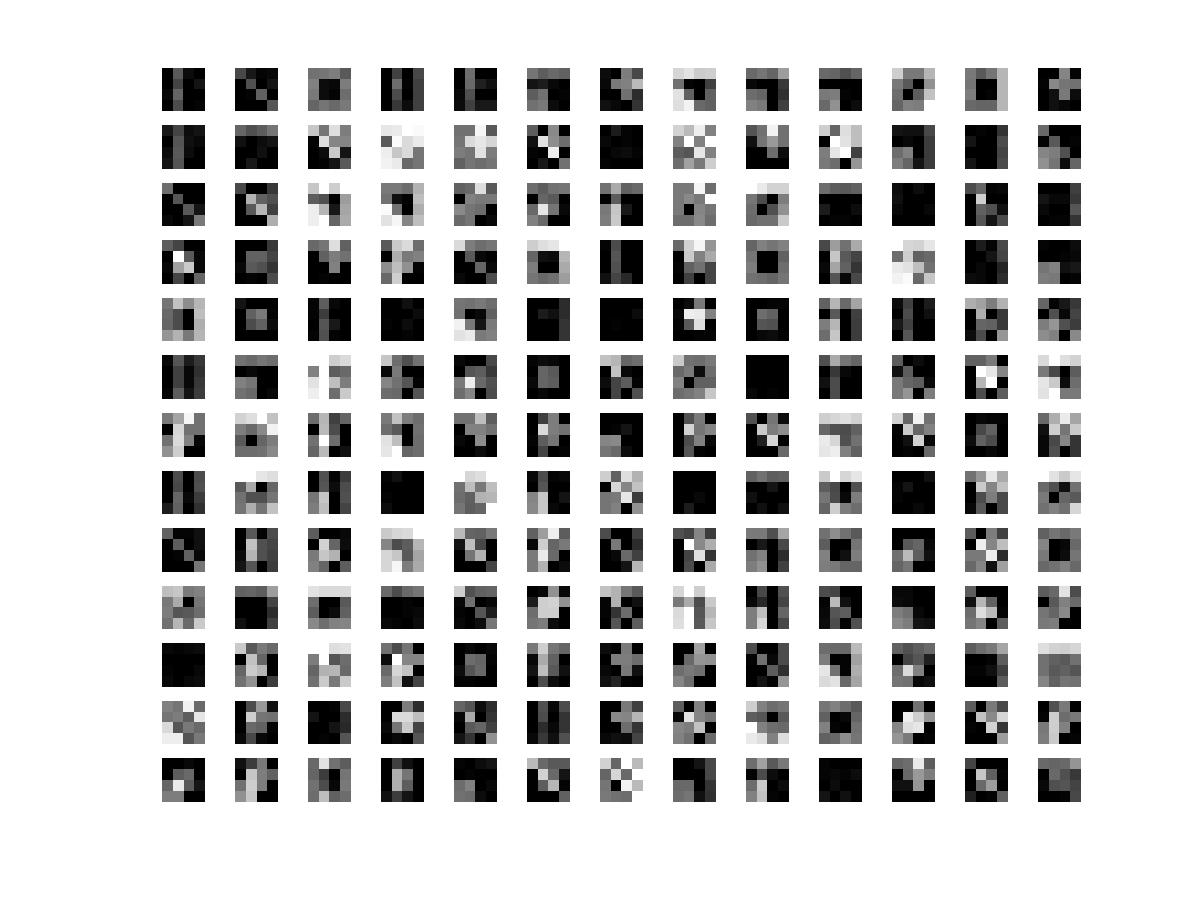
\includegraphics[scale=0.4]{data/images}
\caption{Images generated by randomly combined features with noise}
\label{fig:3d-images}
\end{figure}

Examining the generated images, we can see eight features:
\begin{enumerate}[\hspace{2cm}(1)]
\item a cross
\item a border
\item a two by two square in the middle
\item a two by two square in the bottom left corner
\item a diagonal from top left to bottom right
\item a vertical line in the second column
\item a vertical line in the fourth column
\item a horizontal line in the first row
\end{enumerate}

Factor analysis assumes a model:

\[\textbf{x} = \textbf{W}\textbf{s} + \epsilon\]

where $\epsilon \sim \mathcal{N}(0, \Psi)$ and $\textbf{s} \sim \mathcal{N}(0, \textbf{I})$. Factor analysis would be inappropriate for this data because the our latent variables are binary (i.e. whether or not a feature is present) and not Gaussians.

A mixture of Gaussians assumes as model:

\[\textbf{x} = \sum_{k=1}^K s_k \mu_k + \epsilon \text{ and } \sum_{k=1}^K s_k = 1\]

where $\epsilon \sim \mathcal{N}(0, \Sigma_{\epsilon})$. This also wouldn't be appropriate because it assumes a dirichlet distribution on the vector $\textbf{s}$. Our data is constructed by having each $s_k$ independently sampled from a Bernoulli distribution indicating the presence of feature $\mu_k$.

Independent component analysis assumes a model:

\[\textbf{x} = \textbf{W}\textbf{s} + \epsilon\]

where $\epsilon \sim \mathcal{N}(0, \sigma^2\textbf{I})$ and $P(\textbf{s}) = \prod_{k=1}^K P(s_k)$. This is appropriate for our data because $P(s_k)$ are our independent Bernoulli distributions and we are linearly combining different features with $\textbf{W} \in \mathbb{R}^{D \times K}$and then adding noise $\epsilon$.

Thus, it would be expected that ICA does a good job modelling this data while factor analysis and mixture of Gaussians models would not.

\subsection*{(e)}

We can plot the free energy at each EM step to make sure it increases each iteration:

\begin{figure}[h]
\centering
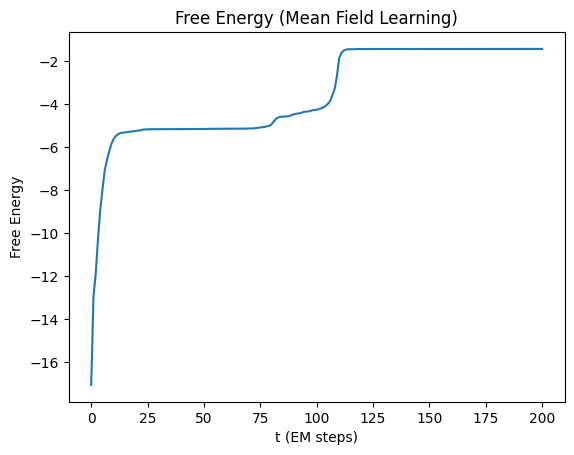
\includegraphics[scale=0.4]{outputs/q3/f-free-energy}
\caption{Free Energy}
\label{fig:3f-free-energy}
\end{figure}
\newpage

\subsection*{(f)}

The initialised features:

\begin{figure}[h]
\centering
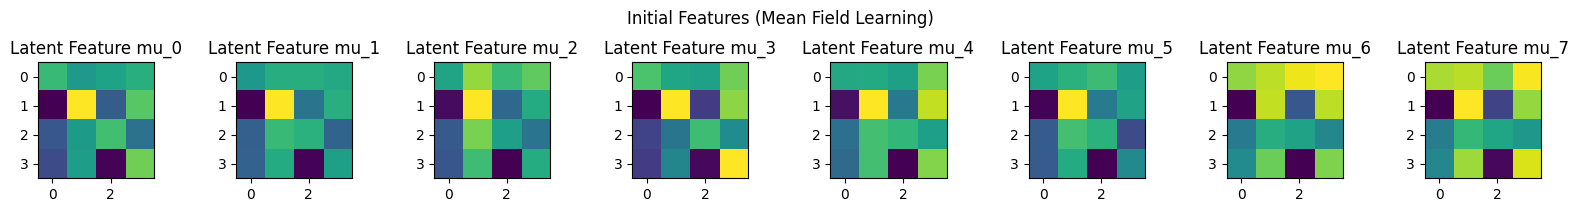
\includegraphics[scale=0.4]{outputs/q3/f-init-latent-factors}
\caption{Initial Latent Factors}
\label{fig:3f-init-latent-factors}
\end{figure}

The features learned by the algorithm:

\begin{figure}[h]
\centering
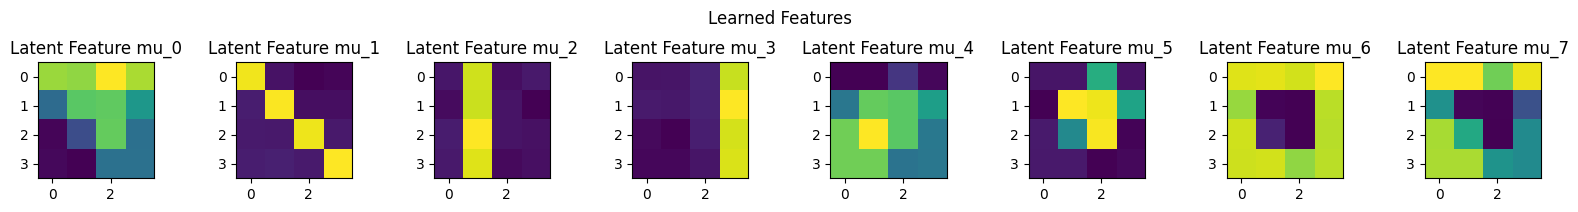
\includegraphics[scale=0.4]{outputs/q3/f-latent-factors}
\caption{Learned Latent Factors}
\label{fig:3f-latent-factors}
\end{figure}

We can see that this approach has learned some of the previously identified features, such as the vertical line in the second column, the two by two square in the bottom left corner, the border, the horizontal line in the first row, and the a two by two square in the middle. The other features seem to be some linear combination of two or more features, such as $\mu_4$ which looks like a combination of the cross and two by two square in the middle.

A possible way to improve our algorithm is reinitialising our algorithm a few times to find better potential convergence results (i.e. choose the model with the highest free energy convergence). We can also increase the number of data samples, with the hopes of learning better features. Finally, we can perform Variational Bayes by setting priors on $\pi$, $\sigma^2$, and $\mu$ for better estimation of these parameters.

When implementing the algorithm, the mean field parameters were initialised randomly, each independently from a uniform distribution on $[ 0, 1]$. $\pi$, $\sigma$, and $\mu$ were initialised by running a maximisation step using these randomly initialised mean field parameters. $K$ was set to eight, after visually identifying eight features in part d. Moreover, for computational stability, when calculating $\log(\lambda_i)$ and $\log(1-\lambda_i)$, we manually shifted $\lambda_i$ by $1e^{-10}$ to prevent $\lambda_i=0$ or $\lambda_i = 1$.


\newpage
\subsection*{(g)}


Plotting the free energy at each partial expectation step of the variational approximation for different $\sigma$'s:

\begin{figure}[h]
\centering
\begin{minipage}{.5\textwidth}
  \centering
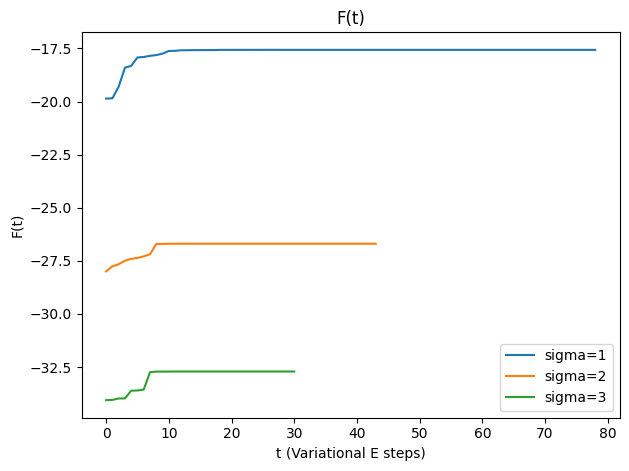
\includegraphics[scale=0.4]{outputs/q3/g-free-energy-sigma}
\caption{Free energy vs $\sigma$}
\label{fig:3g-free-energy-diff-sigma}
\end{minipage}%
\begin{minipage}{.5\textwidth}
  \centering
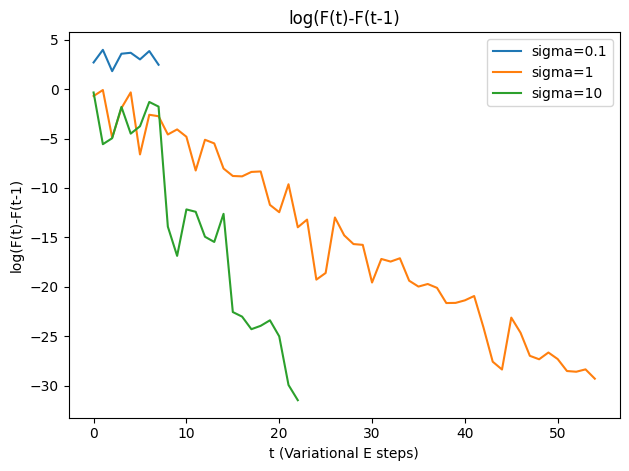
\includegraphics[scale=0.4]{outputs/q3/g-free-energy-diff-sigma}
\caption{Free energy convergence vs $\sigma$}
\label{fig:3g-free-energy-diff-sigma}
\end{minipage}
\end{figure}

We know that our free energy is a upper bounded on the log likelihood:

\[\log P(\mathcal{X} | \theta) \geq \mathcal{F}(q, \theta)\]

In the variational expectation step, $\log P(\mathcal{X} | \theta)$ is fixed by the parameters $\pi$, $\sigma$, and $\mu$ and we adjust our approximation $q$ with parameter $\lambda$ to try to reach this upper bound by increasing $\mathcal{F}(q, \theta)$. We know that $\sigma$ quantifies the noise of $\textbf{x}$, thus a higher $\sigma$ means a wider spread in our distribution $\log P(\mathcal{X} | \theta)$, meaning we are reducing our upper bound for $\mathcal{F}(q, \theta)$. As such, we can see in the plot for free energy above that when $\sigma$ is increased, our free energy converges to a lower value, due to being bounded above by a lower log-likelihood. Moreover, by reducing the upper bound, we see in the plot of $\log(F(t)-F(t-1))$ that our free energy is able to converge faster. Because we have reduced the upper bound by increasing $\sigma$, our free energy reaches the upper bound faster.

\newpage
The Python code for the binary latent factor model:
\lstinputlisting[language=Python]{src/models/binary_latent_factor_models/binary_latent_factor_model.py}

\newpage
The Python code for mean field learning:
\lstinputlisting[language=Python]{src/models/binary_latent_factor_approximations/mean_field_approximation.py}

\newpage
The Python code for expectation maximisation:
\lstinputlisting[language=Python]{src/expectation_maximisation.py}


\newpage
The rest of the Python code for question 3:
\lstinputlisting[language=Python]{src/solutions/q3.py}
\newpage
\section*{Question 4: Variational Bayes for binary factors}
\subsection*{(a)}

To derive a Variational Bayesian hyperparameter optimisation algorithm to automatically determine $K$, the number of hidden binary variables in this model, we begin by writing the expression for $x_d$:

\[P(x_d | \textbf{s}, \textbf{w}_d, \sigma^2) = \mathcal{N}\left(\textbf{s}^T\textbf{w}_d, \sigma^2\right)\]

where we know from the diagonal covariance of $P(\textbf{x} | \textbf{s}, \mu, \sigma^2)$ that each dimension is independent. Moreover, $\textbf{w}_d \in \mathbb{R}^{K\times 1}$, which is the $d^{th}$ row of $\mu \in \mathbb{R}^{D \times K}$

Thus, we can express the posterior as:

\[\log P(\textbf{x}, \textbf{s}, \mu| \pi , \sigma^2,  \alpha) = \log P( \textbf{s}| \pi) + \sum_{d=1}^{D} \log P(x_d | \texbf{s}, \textbf{w}_d, \sigma^2) + \log P( \textbf{w}_d| \alpha)
\]

where we introduce priors on each $\textbf{w}_d$ with $\alpha \in \mathbb{R}^{K \times 1}$.

We choose each prior to be:

\[P( \textbf{w}_d| \alpha) = \mathcal{N}(0, \textbf{A}^{-1})\]

where $\textbf{A} = diag(\alpha)$, the precision matrix.

Combining, we have our expression:

\[
\begin{array}{l}
\log P(\textbf{x}, \textbf{s}, \mu| \pi , \sigma^2,  \alpha) = \sum_{d=1}^D\frac{-1}{2} \log (2 \pi \sigma^2)   -\frac{1}{2 \sigma^2} \left(x_d^2 - 2 x_d \textbf{s}^T \textbf{w}_d   + \textbf{w}_d^T \textbf{s}\textbf{s}^T\textbf{w}_d\right) \\
\tab \tab \tab \tab + \sum_{k=1}^{K} s_k \log \pi_k + (1-s_k) \log (1-\pi_k)}\\
\tab \tab \tab \tab + \sum_{d=1}^D \left( \frac{-K}{2} \log (2 \pi) + \frac{1}{2}  \sum_{k=1}^K \left(\log\alpha_k \right)  -\frac{1}{2}\textbf{w}_{d}^T \textbf{A}\textbf{w}_{d} \right)\\
\end{array}
\]



For the Variational Bayes expectation step, we minimise $\textbf{KL}[q_{\texbf{s}}(\textbf{s} | \text{everything else}) \| P(\textbf{s} | \text{everything else})]$ by setting:

\[q_{\texbf{s}}(\textbf{s}) \propto \exp \left\langle \log P(\textbf{x}, \textbf{s}, \mu| \pi , \sigma^2,  \alpha)  \right\rangle_{q(\mu)}\]

Substituting the relevant terms:

\[q_{\texbf{s}}(\textbf{s}) \propto \exp \left\langle -\frac{1}{2 \sigma^2} \left( - 2 \textbf{x}^T\sum_{k=1}^{K}  s_k  \mu_k   + \sum_{k=1}^{K} \sum_{k'=1, k'\neq k}^{K}  s_k s_{k'} \mu_k^T\mu_{k'} + \sum_{k=1}^{K}  s_k \mu_k^T\mu_k \right) + \sum_{k=1}^{K} s_k \log \frac{\pi_k}{1-\pi_k}\right\rangle_{q(\mu)}\]

Given our factored approximation $q(\textbf{s}) = \prod_{k=1}^K q_k(s_k)$, we can see that we can derive a similar partial update for $q_k(s_k)$ as in Question 3, by taking the variation derivative of the Lagrangian to enforce the normalisation of $q_k$:

\[
\begin{array}{l}
\frac{\partial}{\partial q_k}\left( \exp \left\langle \log P(\textbf{x}, \textbf{s}, \mu| \pi , \sigma^2,  \alpha) \right\rangle_{q(\mu)} + \lambda^{LG} \int q_k -1)\right) \propto \exp \left\langle \log P(\textbf{x}, \textbf{s}, \mu| \pi , \sigma^2,  \alpha) \right\rangle_{q(\mu)\prod_{k'\neq k} q_{k'}(s_{k})} - \log q_k(s_k)\\
\end{array}
\]

Setting this to zero we can solve for $\lambda_i$ where $q_k(s_k) = \lambda_k^{s_k}(1-\lambda_k)^{(1-s_k)}$:

\[ \lambda_k =  \frac{1}{1+\exp\left[ - \left(\frac{  \langle \mu_k\rangle_{q_{\mu_k}}^T}{\sigma^2} \left( \textbf{x} -  \frac{\langle \mu_k\rangle_{q_{\mu_k}}}{2} -  \sum_{k'=1, k'\neq k}^{K}   \lambda_{k'}  \langle \mu_k\rangle_{q_{\mu_k} \right) + \log \frac{ \pi_k}{1- \pi_k\right) \right]}\]

we have our partial E step update.

For the maximisation step, we perform maximisation steps for the parameters $\sigma$ and $\pi$ in the same way as question 3. However, having defined a prior on $\mu$ (through $\textbf{w}$) we will have to derive our expression for $\langle \mu_k\rangle_{q_{\mu_k}}$ the expectation of the posterior on $\mu_k$. This involves deriving the posterior distribution of $\textbf{w}_d$

\[q_{\textbf{w}_d}(\textbf{w}_d})  \propto P(\textbf{w}_d)\exp \left\langle \log P(\textbf{x}, \textbf{s}, \mu| \pi , \sigma^2,  \alpha) \right\rangle_{q_{\textbf{s}}(\textbf{s}) q_{\neg \textbf{w}_d}}\]

Substituting the appropriate terms:

\[q_{\textbf{w}_d}(\textbf{w}_d})\propto \exp\left(-\frac{1}{2}\textbf{w}_{d}^T \textbf{A}\textbf{w}_{d} \right) \exp \left\langle  -\frac{1}{2 \sigma^2} \left(- 2 x_d \textbf{s}^T \textbf{w}_d   + \textbf{w}_d^T \textbf{s}\textbf{s}^T\textbf{w}_d\right)\right\rangle_{q_{\textbf{s}}(\textbf{s}) q_{\neg \textbf{w}_d}}\]

Simplifying:

\[q_{\textbf{w}_d}(\textbf{w}_d})\propto \exp\left(-\frac{1}{2}\left(\textbf{w}_{d}^T \left(\textbf{A}+\frac{\langle  \textbf{s}\textbf{s}^T \rangle_{q_{\textbf{s}}(\textbf{s})}}{\sigma^2} \right)\textbf{w}_{d} - 2 \left(\frac{x_d \langle\textbf{s}^T \rangle_{q_{\textbf{s}}(\textbf{s})}}{\sigma^2}}\right) \textbf{w}_d  \right)\right)\right)\]

We see that the posterior:

\[q_{\textbf{w}_d}(\textbf{w}_d) = \mathcal{N}\left(\mu_{\textbf{w}_d}, \Sigma_{\textbf{w}_d}\right)}\]

where:

\[ \Sigma_{\textbf{w}_d} = \left(\frac{\langle  \textbf{s}\textbf{s}^T \rangle_{q_{\textbf{s}}(\textbf{s})}}{\sigma^2} + \textbf{A}\right)^{-1}\]

and

\[\mu_{\textbf{w}_d} = \Sigma_{\textbf{w}_d}} \left(\frac{x_d \langle\textbf{s}^T \rangle_{q_{\textbf{s}}(\textbf{s})}}{\sigma^2}}\right)\]

Thus, $\langle \mu_k\rangle_{q_{\mu_k}} \in \mathbb{R}^{D \times 1}$ is the concatenation of the $k^{th}$ elements of $\mu_{\textbf{w}_d} \in \mathbb{R}^{K \times 1}$ for $d\in \{1,...,D\}$

For ARD, we must also optimise $\alpha$ with a hyper-M step. We start by choosing $Ga(\alpha_k| a, b)$, a Gamma prior on \alpha_k$, with $a$ and $b$ being hyperparameters. Thus, to optimise $\alpha$ we want to maximise the penalised objective:

\[ \alpha =  \arg \max_{\alpha} \left\langle \log P(\textbf{x}, \textbf{s}, \mu| \pi , \sigma^2,  \alpha) \right\rangle_{q(\textbf{w})} + \sum_{k=1}^K \log P( \alpha_k| a, b)\]

Substituting the appropriate terms, we have our penalised objective $\mathcal{Q}$:

\[\mathcal{Q} =  \left\langle \sum_{d=1}^D \frac{1}{2}  \sum_{k=1}^K \left(\log\alpha_k \right)  -\frac{1}{2}\textbf{w}_{d}^T \textbf{A}\textbf{w}_{d} \right\rangle_{q(\textbf{w})} + \sum_{k=1}^K (a-1)\log\alpha_k -b\alpha_k\]

Simplifying:

\[\mathcal{Q} =  \frac{D}{2}  \sum_{k=1}^K \left( \log\alpha_k \right)  - \frac{1}{2}\sum_{d=1}^D \left( tr \left[ \textbf{A}\left\langle  \textbf{w}_{d}\textbf{w}_{d}^T \right\rangle_{q(\textbf{w}_d)} \right]\right)+ \sum_{k=1}^K (a-1)\log\alpha_k -b\alpha_k\]

Setting $\frac{d\mathcal{Q}}{d\alpha_k} = 0$ we get:

\[ \frac{D}{2\alpha_k} -\frac{1}{2} \sum_{d=1}^D\left\langle (w_{d, k})^2 \right\rangle_{q(\textbf{w}_{d})} + \frac{a-1}{\alpha_k} - b = 0\]

where $w_{d, k}$ is the $k^{th}$ element of $\textbf{w}_d$.

Knowing $\left\langle (w_{d, k})^2 \right\rangle_{q(\textbf{w}_{d})} = (\mu_{\textbf{w}_{d, k}})^2 + \Sigma_{\textbf{w}_{d, (k, k)}}$, the $k^{th}$ element of $\mu_{\textbf{w}_d}$ and element $(k, k)$ of $\Sigma_{\textbf{w}_d$ respectively, we can solve for $\alpha_k$:

\[ \alpha_k = \frac{2a+D-2}{2b+ \sum_{d=1}^D \left((\mu_{\textbf{w}_{d, k}})^2 + \Sigma_{\textbf{w}_{d, (k, k)}}\right) }\]

we have our hyper-M steps for optimising $\alpha$.

\newpage
\subsection*{(b)}

Running variational Bayes for different values of $k$, we can visualise the learned features $\mu_k$ and corresponding $\alpha_k^{-1}$:

\begin{figure}[h]
\centering
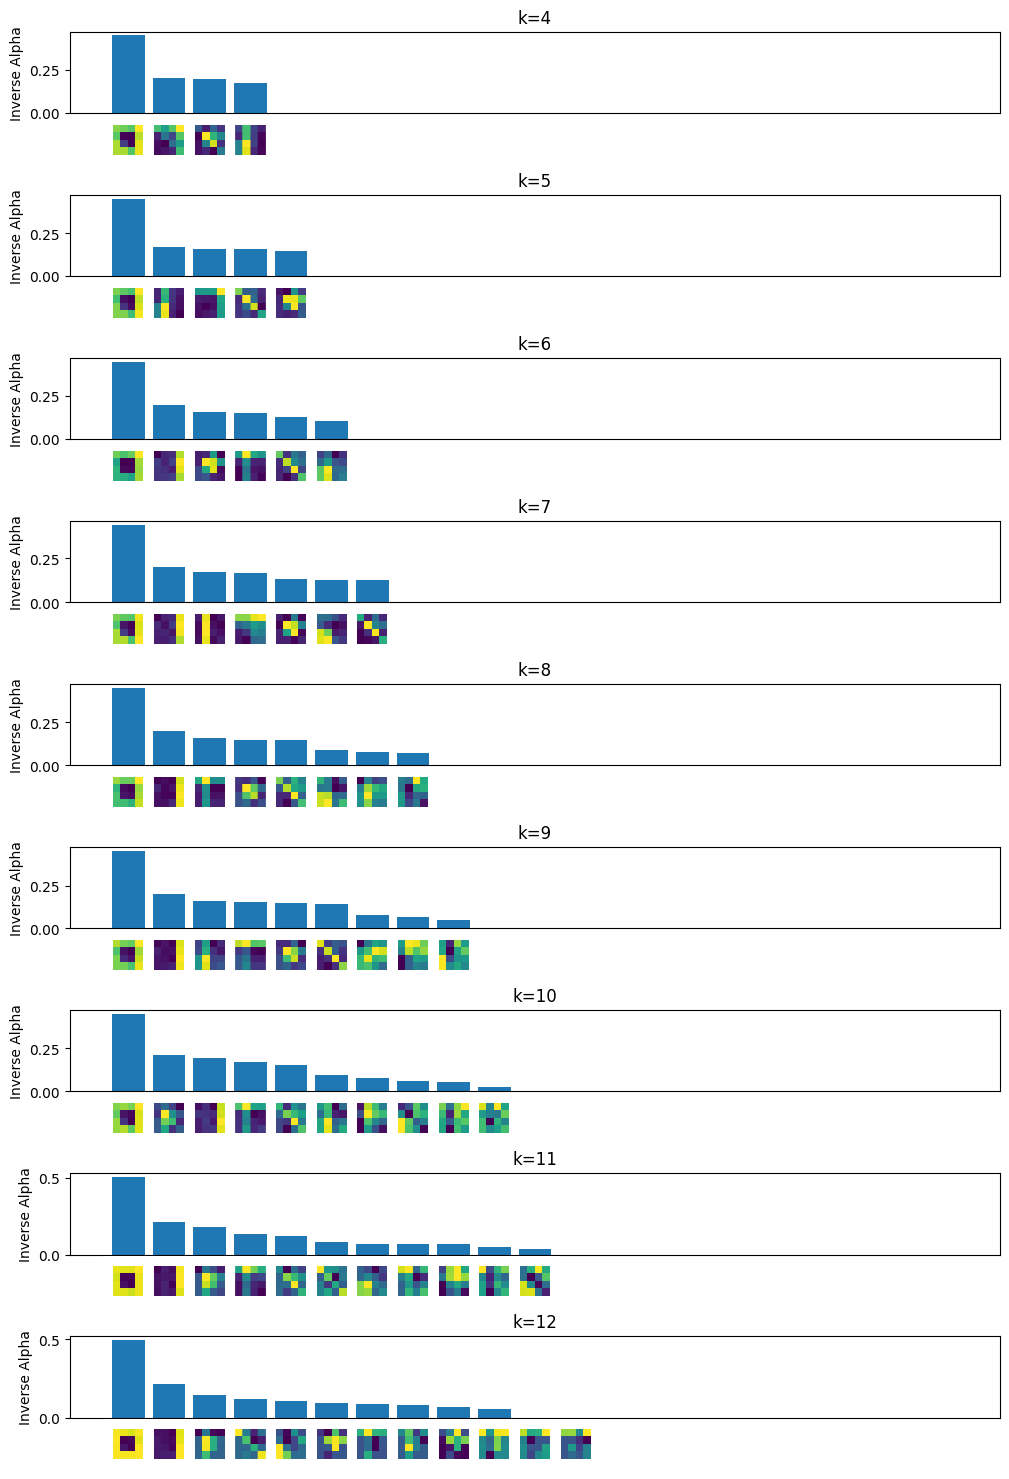
\includegraphics[scale=0.47]{outputs/q4/b-1-latent-factors-comparison}
\caption{Learned Latent Factors vs Inverse Alpha}
\label{fig:}
\end{figure}

\newpage
\begin{figure}[h]
\centering
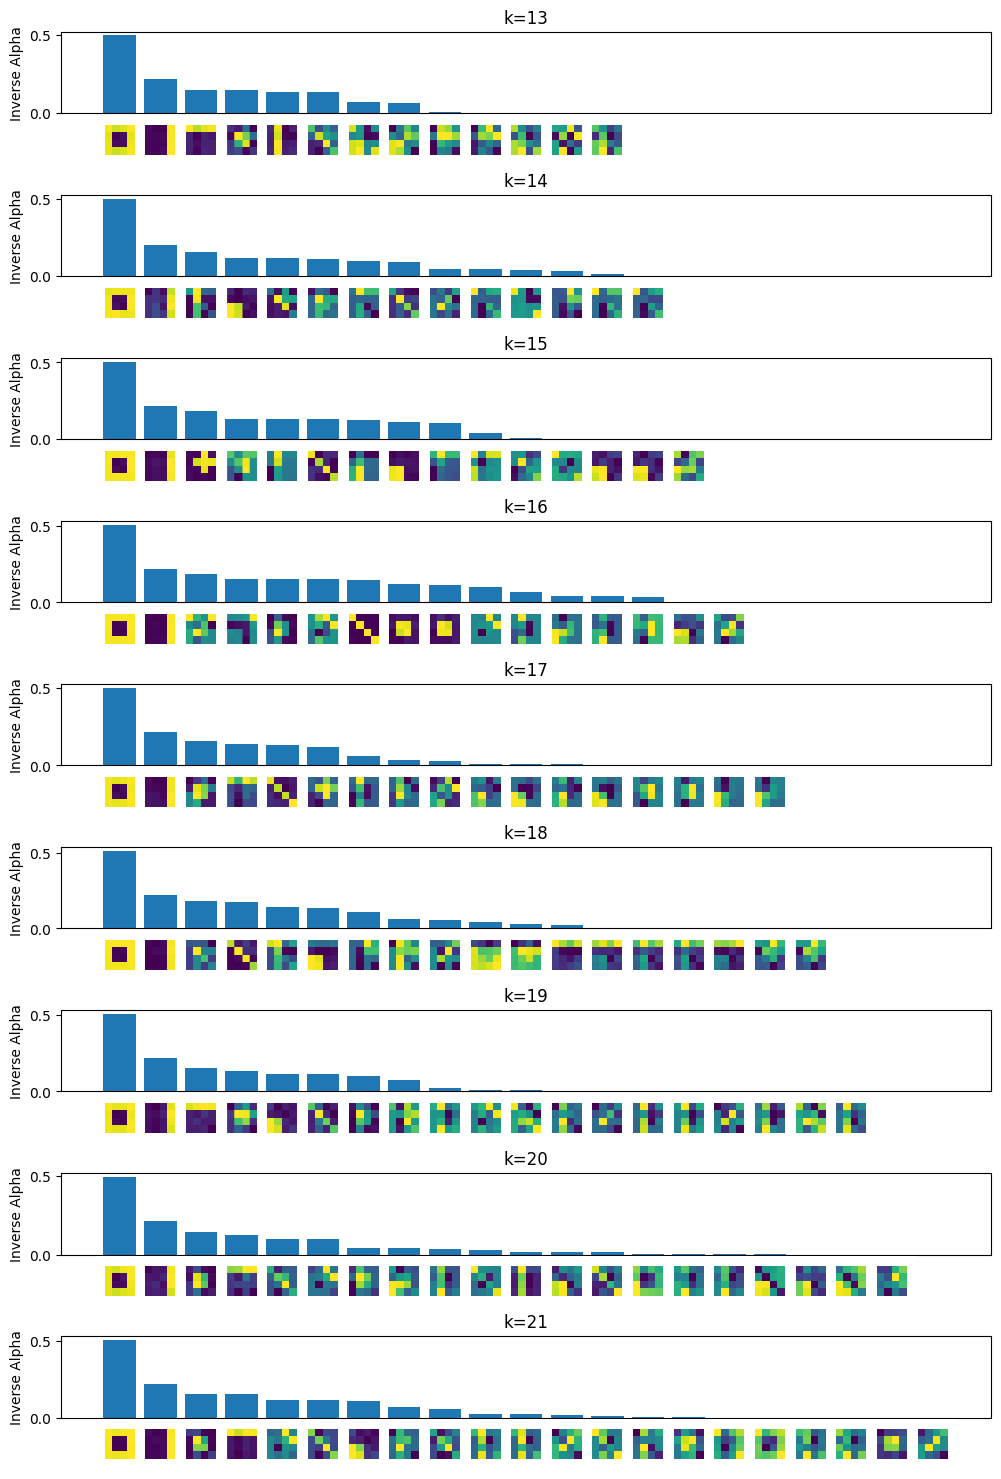
\includegraphics[scale=0.47]{outputs/q4/b-2-latent-factors-comparison}
\caption{Learned Latent Factors vs Inverse Alpha}
\label{fig:}
\end{figure}
As we expect, when running the algorithm for higher $K$ values, many of the features have $\alpha_k \rightarrow \infty$, depicted as $\alpha^{-1}_k \rightarrow 0$ for visual convenience. Moreover, visualising the learned features, we can see the clearest features often have the highest $\alpha^{-1}_k$ while the features deemed irrelevant are often noisy or duplicates.


\newpage

Comparing the free energy plots of models trained on different $K$ values:


\begin{figure}[h]
\centering
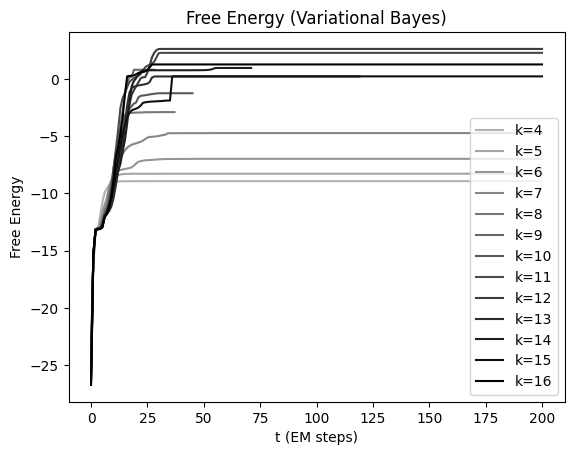
\includegraphics[scale=0.4]{outputs/q4/b-free-energy}
\caption{Free Energy for different values of k}
\label{fig:}
\end{figure}

We can see that initially for $K=4$ to $K=8$, increasing $K$ significantly increases the convergence value of the free energy. However, beyond $K=8$, the trend of $K$ versus the free energy convergence value is not as clear. We can see that this corresponds to the visualisation of $\alpha^{-1}$ where beyond $K=11$, the number of relevant features remains more or less the same. We know that there are only eight latent features, thus models with $K>8$ should be learning duplicate or irrelevant features. As such, we wouldn't expect a model to be able to increase it's free energy significantly when provided with additional degrees of freedom by increasing the value of $K$ beyond eight. We see that for models with $K>>8$, there are typically ten or eleven features that might be deemed relevant (depending on how you threshold) and this is likely from slight overfitting, noise in the data, or duplicate features. Thus, the relationship between the free energy and the effective number of latent features for each model is as we would expect with ARD.


\newpage
The Python code for Variational Bayes:
\lstinputlisting[language=Python]{src/models/binary_latent_factor_models/variational_bayes.py}

\newpage
The Python code for Automatic Relevance Determination:
\lstinputlisting[language=Python]{src/automatic_relevance_determination.py}


\newpage
The rest of the Python code for question 4:
\lstinputlisting[language=Python]{src/solutions/q4.py}


\newpage
\section*{Question 5: EP for the binary factor model}

\subsection*{(a)}

To derive an EP algorithm to infer marginals on the source variables in the binary latent factor model from Question 3, we first write the log-joint probability for a single observation-source pair:

\[\log p(\textbf{s}, \textbf{x}) = \log p(\textbf{s}) + \logp(\textbf{x}|\textbf{s})\]

Knowing $p(\textbf{s}) = \prod_{i=1}^{K}p(s_i| \pi_i)$ and $p(\textbf{x}|\textbf{s}) = \mathcal{N}(\sum_{i=1}^{K} s_i \mu_i, \sigma^2 \textbf{I})$:

\[\log p(\textbf{s}, \textbf{x})  \propto \frac{-1}{2}\left( \textbf{x} - \sum_{i=1}^{K}s_i \mu_i\right)^T \frac{1}{\sigma^2} \textbf{I} \left( \textbf{x} - \sum_{i=1}^{K} s_i \mu_i\right) + \sum_{i=1}^{K} \left(s_i \log\pi_i + (1-s_i)\log(1-\pi_i)\right)\]

Expanding:

\[\log p(\textbf{s}, \textbf{x})  \propto \frac{-1}{2\sigma^2} \left( \textbf{x}^T\textbf{x} - 2\textbf{x}^T\sum_{i=1}^{K}s_i \mu_i + \sum_{i=1}^{K}\sum_{j=1}^{K}s_i s_j \mu_i^T \mu_j\right) + \sum_{i=1}^{K} \left(s_i \log\pi_i + (1-s_i)\log(1-\pi_i)\right)\]

Collecting terms pertaining to $s_i$:

\[\log p(\textbf{s}, \textbf{x})  =    \sum_{i=1}^{K} \left(\left(\frac{\textbf{x}^T \mu_i}{\sigma^2} +\log\frac{\pi_i}{1-\pi_i} \right) s_i\right) + \sum_{i=1}^{K}\sum_{j=1}^{K}\left( \frac{ - \mu_i^T \mu_j}{2\sigma^2} s_i s_j \right) + C\]

where $C$ are all other terms without $s_i$.

Knowing that $s_i^2= s_i$:

\[\log p(\textbf{s}, \textbf{x})  =    \sum_{i=1}^{K} \left(\left(\frac{\textbf{x}^T \mu_i}{\sigma^2} +\log\frac{\pi_i}{1-\pi_i} - \frac{\mu_i^T \mu_i}{2\sigma^2} \right) s_i\right) + \sum_{i=1}^{K}\sum_{j=1}^{i-1}\left( \frac{ - \mu_i^T \mu_j}{\sigma^2} s_i s_j \right) + C\]


Thus:

\[\log p(\textbf{s}, \textbf{x})  =    \sum_{i=1}^{K} \log f_i(s_i) + \sum_{i=1}^{K}\sum_{j=1}^{i-1}\log g_{ij}(s_i, s_j)\right) \]



where the factors are defined:

\[\log f_i(s_i) = \left(\frac{\textbf{x}^T \mu_i}{\sigma^2} +\log\frac{\pi_i}{1-\pi_i} - \frac{\mu_i^T \mu_i}{2\sigma^2} \right) s_i\]

and

\[\log g_{ij}(s_i, s_j) = \frac{- \mu_i^T \mu_j}{\sigma^2} s_i s_j\]

as required.

The Boltzmann Machine can be defined as:

\[P(\textbf{s}| \textbf{W}, \textbf{b}) = \frac{1}{Z} \exp\left( \sum_{i=1}^{K}\sum_{j=1}^{i-1}W_{ij}s_i s_j - \sum_{i=1}^{K} b_i s_i\right)}\]

where $s_i \in \{0, 1\}$, the same as our source variables.

From our factorisation, we can see that $p(\textbf{s}, \textbf{x})$ is a Boltzmann Machine with:

\[W_{ij} = \frac{- \mu_i^T \mu_j}{\sigma^2}\]

and

\[b_i = -\left(\frac{\textbf{x}^T \mu_i}{\sigma^2} +\log\frac{\pi_i}{1-\pi_i} - \frac{\mu_i^T \mu_i}{2\sigma^2}\right)\]

and

\[\log Z = -C \]


\subsection*{(b)}

For $f_i(s_i)$, we will choose a Bernoulli approximation:

\[\tilde{f}_i(s_i) = (\theta_{ii})^{s_i} + (1-\theta_{ii})^{1-s_i}\]


Thus,

\[\log \tilde{f}_i(s_i) \propto \log \left(\frac{\theta_{ii}}{1-\theta_{ii}} \right)s_i\]

we can define $\eta_{ii} = \log \left(\frac{\theta_{ii}}{1-\theta_{ii}} \right)$:

\[\log \tilde{f}_i(s_i) \propto \eta_{ii}s_i\]


For $g_{ij}(s_i, s_j)$, we can choose a product of Bernoulli distributions for our approximation:

\[\tilde{g}_{ij}(s_i, s_j) = \tilde{g}_{ij, \neg s_j}(s_i)\tilde{g}_{ij, \neg s_i}(s_j)\]

where

\[\tilde{g}_{ij, \neg s_j}(s_i) = (\theta_{ji})^{s_i} + (1-\theta_{ji})^{1-s_i}\]

and

\[\tilde{g}_{ij, \neg s_i}(s_j) = (\theta_{ij})^{s_j} + (1-\theta_{ij})^{1-s_j}\]

Thus,

\[\log \tilde{g}_{ij}(s_i, s_j) \propto \log \left(\frac{\theta_{ji}}{1-\theta_{ji}} \right) s_i + \log \left(\frac{\theta_{ij}}{1-\theta_{ij}} \right) s_j\]

we can define $\eta_{ji} = \log \left(\frac{\theta_{ji}}{1-\theta_{ji}} \right)$ and $\eta_{ij} = \log \left(\frac{\theta_{ij}}{1-\theta_{ij}} \right)$:

\[\log \tilde{g}_{ij}(s_i, s_j) \propto \eta_{ji} s_i + \eta_{ij} s_j\]


To derive a message passing scheme, we define the incoming message to node $i$ from the singleton factor:

\[\mathcal{M}_{i \rightarrow i}(s_i) = \tilde{f}_i(s_i)\]

and the incoming message to node $i$ from node $j$:

%\[\mathcal{M}_{j \rightarrow i} = \sum_{\substack{s_m \in \{0, 1\} \\ m \in \{1, ..., j-1, j+1,... K\}}} \tilde{f}_j(s_j) \prod_{k\in ne(j), k\neq i}^{K}} g_{kj}(s_k, s_j)\]

%\[\mathcal{M}_{j \rightarrow i}(s_i) = \sum_{s_1 \in \{0, 1\} } \cdots \sum_{s_{i-1} \in \{0, 1\} } \sum_{s_{i+1} \in \{0, 1\} } \cdots \sum_{s_1 \in \{0, 1\} } \tilde{f}_j(s_j) \tilde{g}_{ji}(s_j, s_i) \prod_{k\in ne(j), k\neq i}^{K}} \tilde{g}_{kj}(s_k, s_j)\]


\[\mathcal{M}_{j \rightarrow i}(s_i) = \sum_{s_1 \in \{0, 1\} } \cdots \sum_{s_{i-1} \in \{0, 1\} } \sum_{s_{i+1} \in \{0, 1\} } \cdots \sum_{s_1 \in \{0, 1\} }  \tilde{g}_{ji}(s_j, s_i) \mathcal{M}_{j \rightarrow j}(s_j)\prod_{k\in ne(j), k\neq i}^{K}} \mathcal{M}_{k \rightarrow j}(s_j)\]

where $ne(j)$ are indices of neighbouring nodes of node $j$. This is the product of the incoming messages to node $j$ from its neighbours, the singleton message from node $j$, and $\tilde{g}_{ji}(s_j, s_i)$ with all nodes except $s_i$ marginalised out.

Because $\tilde{g}_{ji}(s_j, s_i)$ is a product:

\[\mathcal{M}_{j \rightarrow i}(s_i) = \tilde{g}_{ji, \neg s_j}(s_i) \sum_{s_1 \in \{0, 1\} } \cdots \sum_{s_{i-1} \in \{0, 1\} } \sum_{s_{i+1} \in \{0, 1\} } \cdots \sum_{s_1 \in \{0, 1\} } \tilde{f}_j(s_j) \tilde{g}_{ji, \neg s_i}(s_j) \prod_{k\in ne(j), k\neq i}^{K}} \mathcal{M}_{k \rightarrow j}(s_j)\]

We are left with:

\[\mathcal{M}_{j \rightarrow i}(s_i) = \tilde{g}_{ji, \neg s_j}(s_i)\]

and

\[\mathcal{M}_{j \rightarrow i}(s_i) \propto \exp\left(\eta_{ji} s_i\right)\]



The cavity distributions are:

\[q_{\neg \tilde{f}_i(s_i)}(s_i) =
\prod_{j\in ne(i)}^{K} \mathcal{M}_{j \rightarrow i}(s_i)
\]

and

\[q_{\neg \tilde{g}_{ij}(s_i, s_j)}(s_i, s_j) = \left( \mathcal{M}_{i \rightarrow i}(s_i) \prod_{k\in ne(i), k\neq j}^{K} \mathcal{M}_{k \rightarrow i}(s_i)
\right)\left( \mathcal{M}_{j \rightarrow j}(s_j) \prod_{k\in ne(j), k\neq i}^{K} \mathcal{M}_{k \rightarrow j}(s_j)
\right)
\]

For $\tilde{f}_{i}(s_{i})$, we do not need to make an approximation step.
This is because we are minimising:

\[\tilde{f}_{i}(s_{i}) = \arg \min_{\tilde{f}_{i}(s_{i})} \textbf{KL} \left[ f_{i}(s_{i}) q_{\neg \tilde{f}_i(s_i)}(s_i) \| \tilde{f}_{i}(s_{i}) q_{\neg \tilde{f}_i(s_i)}(s_i) \right]\]

We know that the factor $\log f_i(s_i)$ is a Bernoulli of the form $b_i s_i$. Because our approximation for this site is also Bernoulli, we can simply solve for $\theta_{ii}$ in $\log \tilde{f}_{i}(s_{i})$:

\[\log \tilde{f}_i(s_i) = \log f_{i}(s_{i})\]


\[\log \left(\frac{\theta_{ii}}{1-\theta_{ii}} \right)s_i = b_i s_i\]

\[\theta_{ii} = \frac{1}{1+\exp(-b_i)}\]

On the other hand, for $\tilde{g}_{ij}(s_i, s_j)$, we will approximate with:

\[\tilde{g}_{ij}(s_i, s_j) = \arg \min_{\tilde{g}_{ij}(s_i, s_j)} \textbf{KL} \left[ g_{ij}(s_i, s_j) q_{\neg \tilde{g}_{ij}(s_i, s_j)}(s_i, s_j) \left\| \tilde{g}_{ij}(s_i, s_j) q_{\neg \tilde{g}_{ij}(s_i, s_j)}(s_i, s_j) \right]\]

We can define natural parameters $\eta_{i, \neg s_j}$ and $\eta_{j, \neg s_i}$ for $q_{\neg \tilde{g}_{ij}(s_i, s_j)}(s_i, s_j)$ such that:

\[\mathcal{M}_{i \rightarrow i}(s_i) \prod_{k\in ne(i), k\neq j}^{K} \mathcal{M}_{k \rightarrow i}(s_i) \propto \exp(\eta_{i, \neg s_j} s_i)\]

\[ \mathcal{M}_{j \rightarrow j}(s_j) \prod_{k\in ne(j), k\neq j}^{K} \mathcal{M}_{k \rightarrow j}(s_j) \propto \exp(\eta_{j, \neg s_i} s_j)\]

Note that $\tilde{g}_{ij}(s_i, s_j)$ was chosen as the product of two Bernoulli distributions, so updates to this site approximation involves updating the  parameters $\eta_{ji}$ and $\eta_{ij}$, for $s_i$ and $s_j$ respectively.

We can write:
%\[\log \tilde{g}_{ij}q_{\neg \tilde{g}_{ij}} \propto \log \left(\frac{\theta_i}{1-\theta_i} \right) s_i + \log \left(\frac{\theta_j}{1-\theta_j} \right) s_j + \sum_{i=1}^{K}  \log \left(\frac{\theta_{ii}}{1-\theta_{ii}} \right) +  \sum_{i'=1}^{K}\sum_{\substack{j'=1 \\ i', j' \neq i, j}}^{i'-1}  \log \left(\frac{\theta_i}{1-\theta_i} \right) s_i + \log \left(\frac{\theta_j}{1-\theta_j} \right) s_j\]

\[\log \left(\tilde{g}_{ij}(s_i, s_j)q_{\neg \tilde{g}_{ij}(s_i, s_j)}(s_i, s_j)\right) \propto \eta_{ji} s_i + \eta_{ij} s_j + \eta_{i, \neg s_j} s_i + \eta_{j, \neg s_i} s_j\]

Simplifying:

\[\log \left(\tilde{g}_{ij}(s_i, s_j) q_{\neg \tilde{g}_{ij}(s_i, s_j)}(s_i, s_j) \right)\propto \left(\eta_{ji}+ \eta_{i, \neg s_j} \right) s_i + \left(\eta_{ij} + \eta_{j, \neg s_i} \right) s_j \]


Thus, the first moments:

\[\mathbb{E}_{s_i}\left[\sum_{s_j \in \{0, 1\}}\tilde{g}_{ij}(s_i, s_j) q_{\neg \tilde{g}_{ij}(s_i, s_j)}(s_i, s_j)\right] = \frac{1}{1+\exp{\left(-\left(\eta_{ji} + \eta_{i, \neg s_j} \right)}\right)}\]

and

\[\mathbb{E}_{s_j}\left[\sum_{s_i \in \{0, 1\}}\tilde{g}_{ij}(s_i, s_j) q_{\neg \tilde{g}_{ij}(s_i, s_j)}(s_i, s_j)\right] = \frac{1}{1+\exp{\left(-\left(\eta_{ij} + \eta_{j, \neg s_i} \right)}\right)}\]

Moreover:

\[\log \left(g_{ij}(s_i, s_j) q_{\neg \tilde{g}_{ij}(s_i, s_j)}(s_i, s_j) \right)\propto W_{ij} s_i s_j
 + \eta_{i, \neg s_j} s_i + \eta_{j, \neg s_i} s_j\]

To derive the first moment for $ g_{ij}(s_i, s_j) q_{\neg \tilde{g}_{ij}(s_i, s_j)}(s_i, s_j)$ with respect to $s_i$, we first marginalise out $s_j$:

\[ \sum_{s_j \in \{0, 1\}} g_{ij}(s_i, s_j) q_{\neg \tilde{g}_{ij}(s_i, s_j)}(\textbf{s}) \propto \exp\left( W_{ij} s_i + \eta_{i, \neg s_j} s_i + \eta_{j, \neg s_i}\right) +  \exp\left(\eta_{i, \neg s_j} s_i \right)
\]

Thus, the first moment:

\[\mathbb{E}_{s_i}\left[\sum_{s_j \in \{0, 1\}}g_{ij}(s_i, s_j) q_{\neg \tilde{g}_{ij}(s_i, s_j)}(s_i, s_j)\right] = \frac{\exp\left( W_{ij} + \eta_{i, \neg s_j}  + \eta_{j, \neg s_i}\right) +  \exp\left(\eta_{i, \neg s_j}\right)}{\left[\exp\left( W_{ij} + \eta_{i, \neg s_j}  + \eta_{j, \neg s_i}\right) +  \exp\left(\eta_{i, \neg s_j}\right)\right]+\left[\exp\left( \eta_{j, \neg s_i}\right) +  1\right]}\]

Simplifying:

\[\mathbb{E}_{s_i}\left[\sum_{s_j \in \{0, 1\}}g_{ij}(s_i, s_j) q_{\neg \tilde{g}_{ij}(s_i, s_j)}(s_i, s_j)\right] = \frac{\exp\left(\eta_{i, \neg s_j}\right)\left(\exp\left( W_{ij}  + \eta_{j, \neg s_i}\right) + 1\right)  }{\left[\exp\left(\eta_{i, \neg s_j}\right)\left(\exp\left( W_{ij}  + \eta_{j, \neg s_i}\right) + 1\right)  \right]+\left[\exp\left( \eta_{j, \neg s_i}\right) +  1\right]}\]

Similarly:

\[\mathbb{E}_{s_j}\left[\sum_{s_i \in \{0, 1\}}g_{ij}(s_i, s_j) q_{\neg \tilde{g}_{ij}(s_i, s_j)}(s_i, s_j)\right] = \frac{\exp\left(\eta_{j, \neg s_i}\right)\left(\exp\left( W_{ij}  + \eta_{i, \neg s_j}\right) + 1\right)  }{\left[\exp\left(\eta_{j, \neg s_i}\right)\left(\exp\left( W_{ij}  + \eta_{i, \neg s_j}\right) + 1\right) \right]+\left[\exp\left( \eta_{i, \neg s_j}\right) +  1\right]}\]


By setting:

\[\mathbb{E}_{s_i}\left[\sum_{s_j \in \{0, 1\}}\tilde{g}_{ij}(s_i, s_j) q_{\neg \tilde{g}_{ij}(s_i, s_j)}(s_i, s_j)\right] = \mathbb{E}_{s_i}\left[\sum_{s_j \in \{0, 1\}}g_{ij}(s_i, s_j) q_{\neg \tilde{g}_{ij}(s_i, s_j)}(s_i, s_j)\right]\]


and

\[\mathbb{E}_{s_j}\left[\sum_{s_i \in \{0, 1\}}\tilde{g}_{ij}(s_i, s_j) q_{\neg \tilde{g}_{ij}(s_i, s_j)}(s_i, s_j)\right] = \mathbb{E}_{s_j}\left[\sum_{s_i \in \{0, 1\}}g_{ij}(s_i, s_j) q_{\neg \tilde{g}_{ij}(s_i, s_j)}(s_i, s_j)\right]\]

we can solve for the parameters of $\tilde{g}_{ij}(s_i, s_j)$ with moment matching:

\[\frac{1}{1+\exp{\left(-\left(\eta_{ji} + \eta_{i, \neg s_j} \right)}\right)}} = \frac{\exp\left(\eta_{i, \neg s_j}\right)\left(\exp\left( W_{ij}  + \eta_{j, \neg s_i}\right) + 1\right)  }{\left[\exp\left(\eta_{i, \neg s_j}\right)\left(\exp\left( W_{ij}  + \eta_{j, \neg s_i}\right) + 1\right)  \right]+\left[\exp\left( \eta_{j, \neg s_i}\right) +  1\right]}\]

Simplifying:

\[\exp\left( \eta_{j, \neg s_i}\right) +  1=\exp{\left(-\left(\eta_{ji} + \eta_{i, \neg s_j} \right)}\right)}\exp\left(\eta_{i, \neg s_j}\right)\left(\exp\left( W_{ij}  + \eta_{j, \neg s_i}\right) + 1\right)\]

\[\frac{\exp\left( \eta_{j, \neg s_i}\right) +  1}{ \exp\left( W_{ij}  + \eta_{j, \neg s_i}\right) + 1} =\exp{\left(-\eta_{ji}\right)}\]

Our parameter update:

\[\eta_{ji} = \log \left( \frac{1+\exp\left( W_{ij}  + \eta_{j, \neg s_i}\right)}{1+\exp\left( \eta_{j, \neg s_i}\right)} \right)\]

Similarly:

\[\eta_{ij} = \log \left( \frac{1+\exp\left( W_{ij}  + \eta_{i, \neg s_j}\right)}{1+\exp\left( \eta_{i, \neg s_j}\right)} \right)\]


\subsection*{(c)}

Using factored approximate messages, we see that:

\[\eta_{i, \neg s_j} =  \log \left(\frac{\theta_{ii}}{1-\theta_{ii}}\right) + \sum_{k\in ne(i), k\neq j}^{K} \log\left(\frac{\theta_{ki}}{1-\theta_{ki}} \right)\]

Knowing $\eta_{ii}=\log \left(\frac{\theta_{ii}}{1-\theta_{ii}}\right)$ and $\eta_{ki}=\log\left(\frac{\theta_{ki}}{1-\theta_{ki}} \right)$:

\[\eta_{i, \neg s_j} =  \eta_{ii} + \sum_{k\in ne(i), k\neq j}^{K} \eta_{ki}\]

and

\[\eta_{j, \neg s_i} =  \eta_{jj} + \sum_{k\in ne(j), k\neq i}^{K} \eta_{kj}\]


The summation of the natural parameters of the singleton factor for node $i$ with the natural parameters of messages from all the neighbouring nodes that aren't $j$.

This leads to a loopy BP algorithm because the nodes are fully connected (i.e. every node is the neighbour of all other nodes). Thus, we cannot simply move from one end of the graph to the other like BP for tree structured graphs.

Moreover, our factored approximations:

\[q(s_i) \propto \sum_{j=1}^{K} \eta_{ij} s_i\]

and so:

\[\lambda_i = \frac{1}{1+\exp(-\sum_{j=1}^{K} \eta_{ij})}\]

our parameter for $q(s_i)$.


\newpage
\subsection*{(d)}

We can use automatic relevance determination (ARD) as a hyperparameter method to select relevant features by placing a prior on $\mu_k$ in the same way as Question 4. With a hyper-M step, certain features will have diverging precision, leaving us with the relevant features, from which we get our $K$. We can implement this by running the message passing algorithm (loopy BP) which was implemented for Question 6 for the expectation step and the VB algorithm for the maximisation step (along with its hyper-M Step) which was implemented for Question 4:

\begin{figure}[h]
\centering
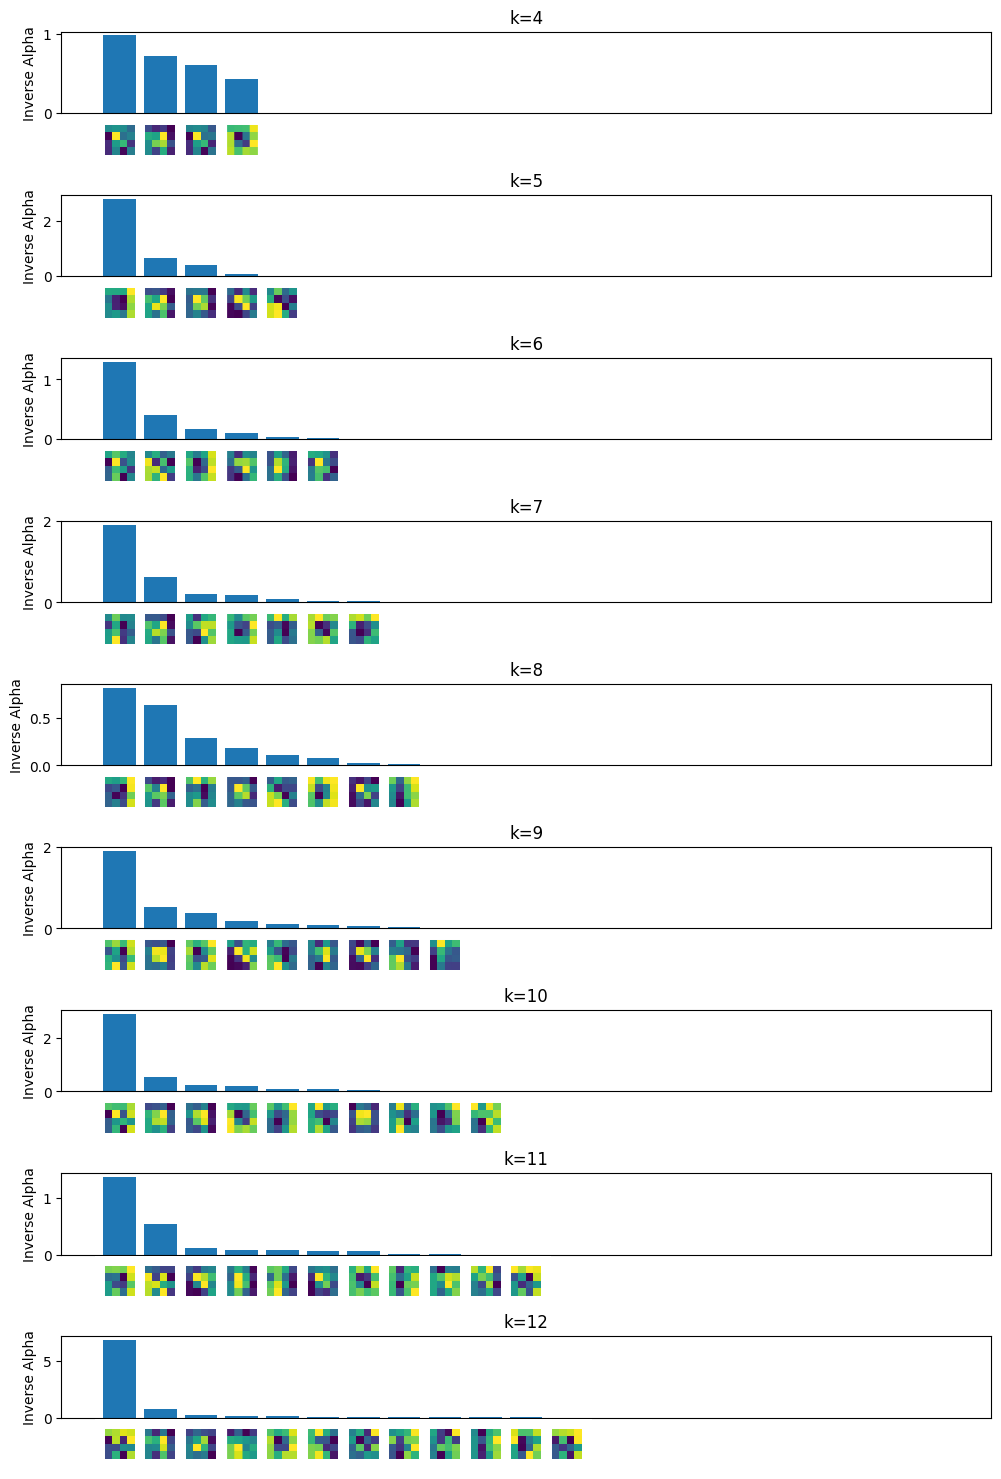
\includegraphics[scale=0.47]{outputs/q5/d-1-latent-factors-comparison}
\caption{Learned Latent Factors vs Inverse Alpha}
\label{fig:}
\end{figure}

\newpage
\begin{figure}[h]
\centering
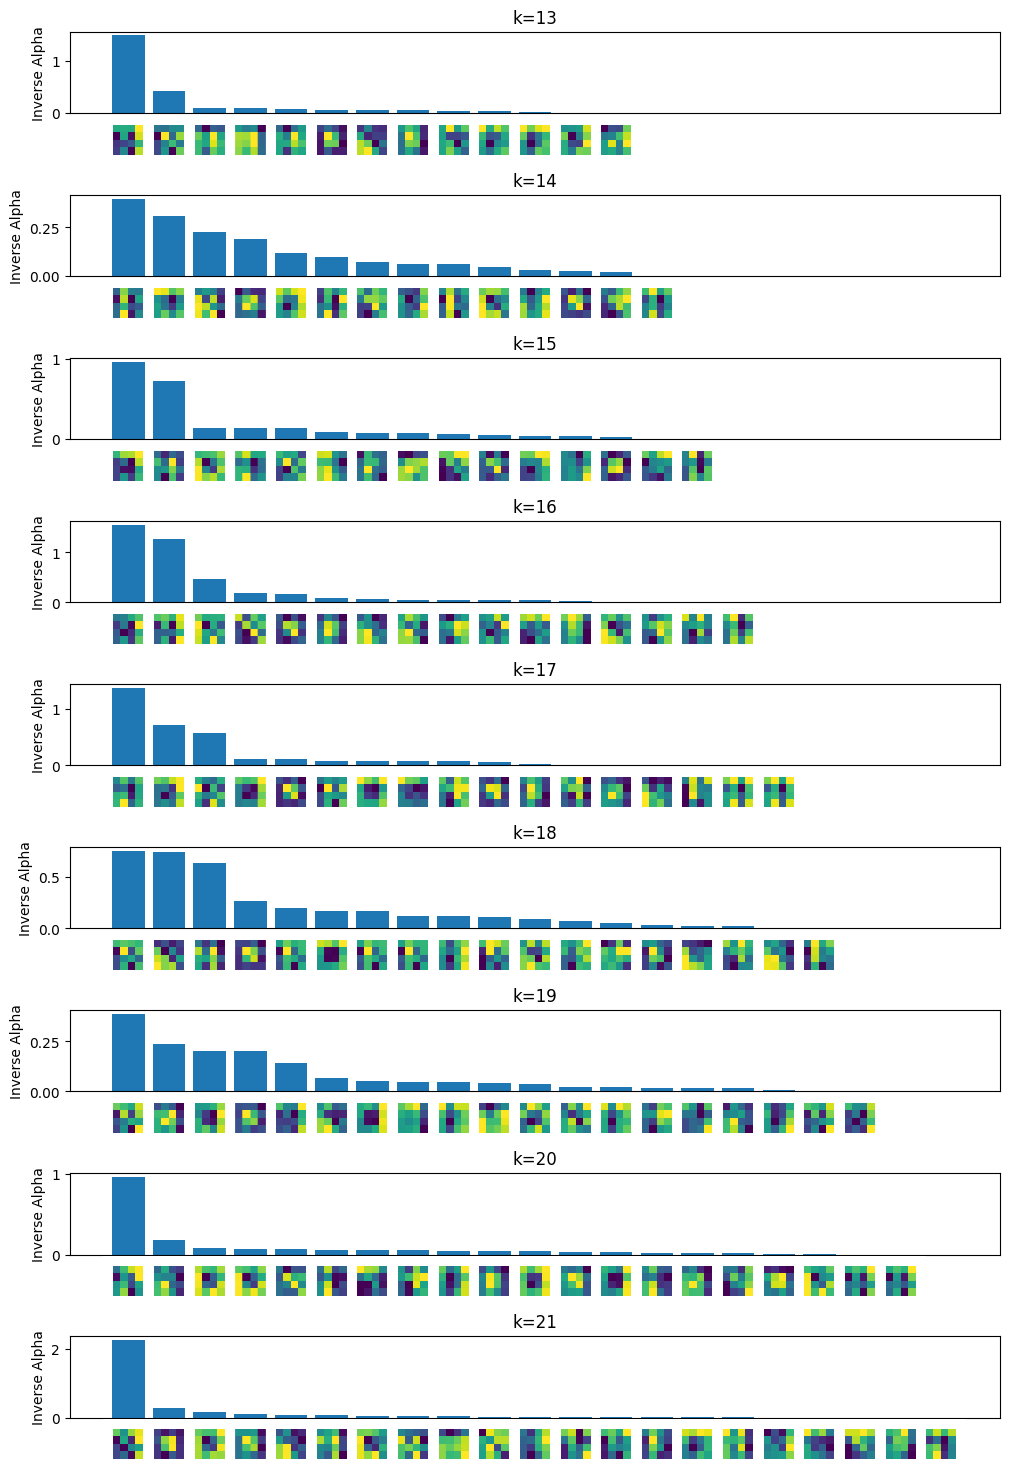
\includegraphics[scale=0.47]{outputs/q5/d-2-latent-factors-comparison}
\caption{Learned Latent Factors vs Inverse Alpha}
\label{fig:}
\end{figure}

We can see that ARD has more difficulty finding relevant features when using loop BP.
However, looking at the features themselves, we can see that the features are not very clear compared those from the mean field approximation or Variational Bayes in Question 4.
This is probably why we do not consistently have the same number of $\alpha_k$ values that don't diverge as compared with Question 4.
Moreover we usually have fewer than eight features that don't converge, likely because loopy BP seems to be unable to identify too many clear features that we would want to deem relevant in the first place.
However, we can see for $K<8$ that more of the features are deemed relevant as we would expect.

\newpage
Comparing the free energy plots of models trained on different $K$ values:

\begin{figure}[h]
\centering
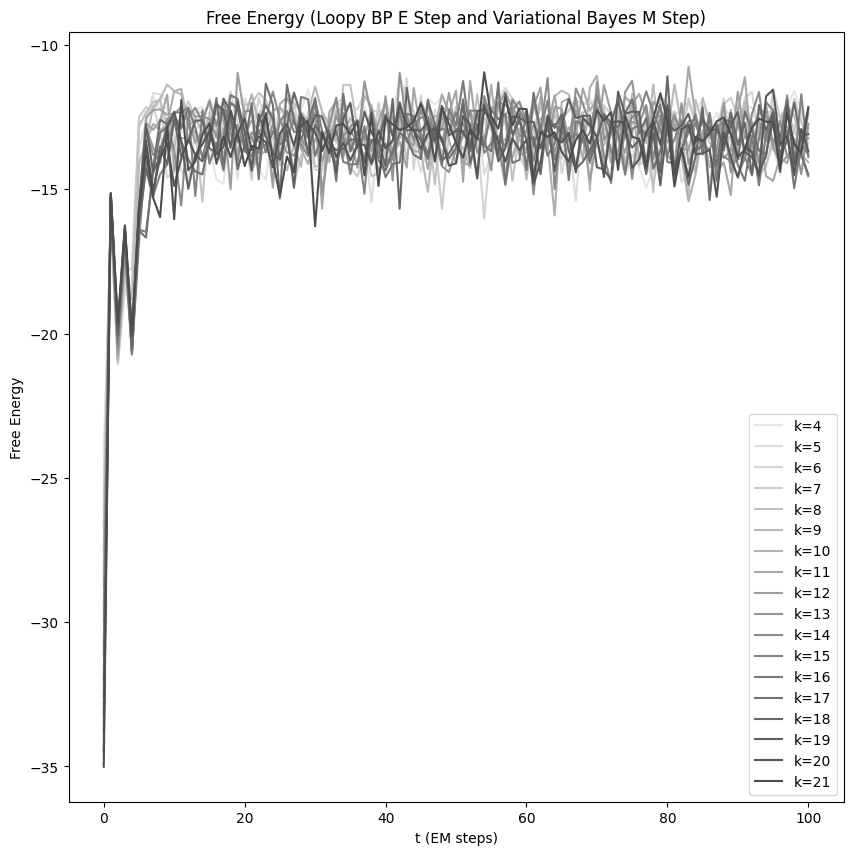
\includegraphics[scale=0.4]{outputs/q5/d-free-energy}
\caption{Free Energy for different values of k}
\label{fig:}
\end{figure}

We can see the difficulties of this approach due to the inability for loopy BP to converge for this particular problem.
This likely contributes to the difficulty for ARD to find relevant features when the message passing algorithm is unable to converge on generating meaningful features.
To improve this, we could also put priors on the other parameters $\sigma^2$ and $\pi$ in the hopes that this will help stabilise the algorithm.
Moreover, because loopy BP is unable to converge for this problem, it is quite computationally intensive as EM will always run the maximum number of iterations without improvement in the results.
Knowing that it won't converge, employing early stopping or fewer iterations can also be helpful.
Moreover, Boltzmann machines do not scale well with respect to the number of nodes, $K$, introducing computational difficulties.
This was experienced when generating the above results, where for larger $K$ values, loopy BP E steps took much longer to perform. To tackle this, a restricted Boltzmann Machine could be implemented to reduce the number of connections in the graph, alleviating these computational difficulties.


\newpage
The Python code for question 5:
\lstinputlisting[language=Python]{src/solutions/q5.py}


\newpage
\section*{Question 6: EP/Loopy BP Implementation}

Implementing the EP/loopy-BP algorithm, we can compare the learned latent factors with those of the variational mean-field algorithm:

\begin{figure}[h]
\centering
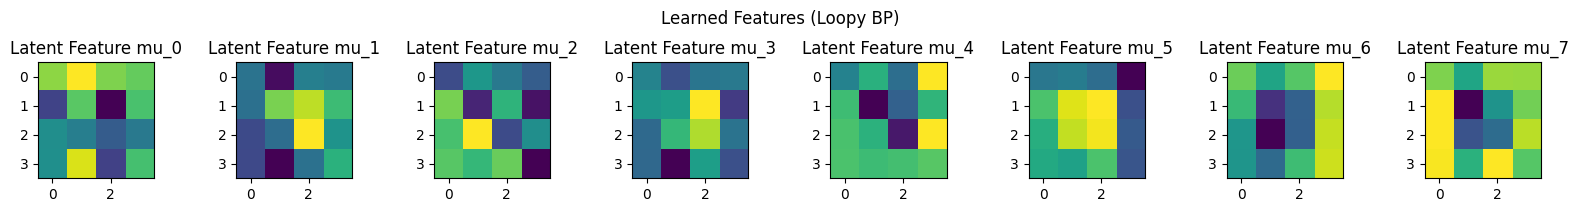
\includegraphics[scale=0.4]{outputs/q6/all-latent-factors}
\caption{Learned Latent factors learned with EP/Loopy-BP}
\label{fig:6-latent-factors}
\end{figure}

\begin{figure}[h]
\centering
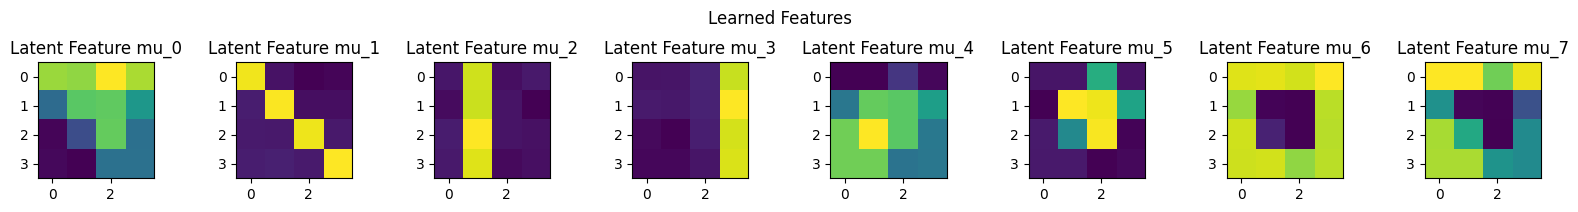
\includegraphics[scale=0.4]{outputs/q3/f-latent-factors}
\caption{Learned Latent Factors with Mean Field Approximation}
\label{fig:3f-latent-factors}
\end{figure}

We can see that the mean field algorithm seems to learn better latent features. In particular there are fewer duplicates, unlike loopy BP that has a few duplicates. Moreover, the learned features of the mean field algorithm have less noise than those from loopy BP. For example $\mu_0$ for the mean field algorithm looks almost like a binary image. We can understand the reason for this by comparing the free energies of the two algorithms:

\begin{figure}[h]
\centering
\begin{minipage}{.5\textwidth}
  \centering
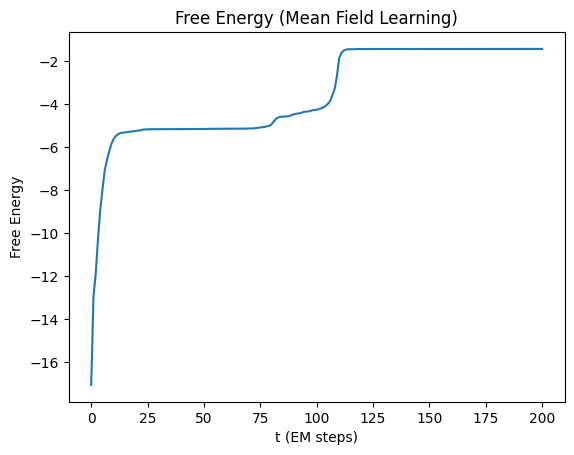
\includegraphics[scale=0.4]{outputs/q3/f-free-energy}
\caption{Mean Field Approximation}
\label{fig:3g-free-energy-diff-sigma}
\end{minipage}%
\begin{minipage}{.5\textwidth}
  \centering
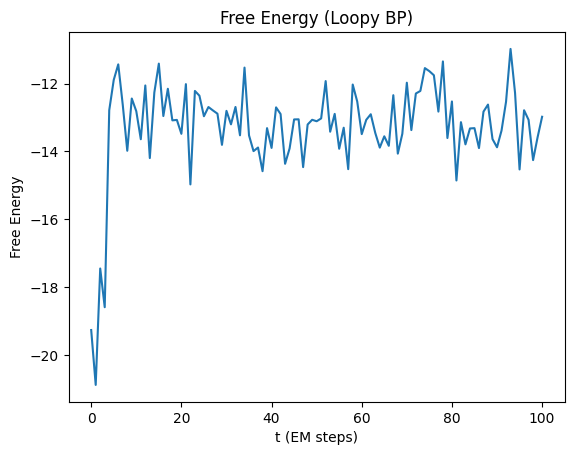
\includegraphics[scale=0.4]{outputs/q6/all-free-energy}
\caption{Loopy BP}
\label{fig:3g-free-energy-diff-sigma}
\end{minipage}
\end{figure}

We can observe that the free energy of the mean field algorithm converges while our loopy belief propagation is unable to converge to a free energy. Because loopy BP does not have convergence guarantees, one of the limitations of this approach, we can see that in this case loopy BP is unable to identify many latent factors.

\newpage
The Python code for the Boltzmann machine:
\lstinputlisting[language=Python]{src/models/binary_latent_factor_models/boltzmann_machine.py}

\newpage
The Python code for message passing:
\lstinputlisting[language=Python]{src/models/binary_latent_factor_approximations/message_passing_approximation.py}

\newpage
The rest of the Python code for question 6:
\lstinputlisting[language=Python]{src/solutions/q6.py}

\newpage
\section*{Appendix 1: abstract\_binary\_latent\_factor\_model.py}
\lstinputlisting[language=Python]{src/models/binary_latent_factor_models/abstract_binary_latent_factor_model.py}
\newpage
\section*{Appendix 2: abstract\_binary\_latent\_factor\_approximation.py}
\lstinputlisting[language=Python]{src/models/binary_latent_factor_approximations/abstract_binary_latent_factor_approximation.py}
\newpage
\section*{Appendix 3: main.py}
\lstinputlisting[language=Python]{main.py}
\newpage
\section*{Appendix 4: constants.py}
\lstinputlisting[language=Python]{src/constants.py}
\section*{Appendix 5: generate\_images.py}
\lstinputlisting[language=Python]{src/generate_images.py}
\newpage
\section*{Appendix 6: m\_step.py}
\lstinputlisting[language=Python]{demo_code/m_step.py}
\end{document}